\documentclass[11pt,a4paper]{article}

\usepackage[T1]{fontenc}
\usepackage{lmodern}
\usepackage{geometry}
\usepackage{booktabs}
\usepackage{longtable}
\usepackage{hyperref}
\usepackage{graphicx}
\usepackage{siunitx}
\usepackage{amsmath}
\usepackage{color}
\usepackage{enumitem}
\usepackage{verbatim}
\usepackage{authblk}
\usepackage{float}

\geometry{margin=2.5cm}
\setlist{noitemsep}

\title{Qualification of the OpenMC Radiation Transport Code for ITER}

\author[1]{Bor Kos}
\author[2]{Aljaz Kolsek}
\author[3]{Alex Valentine}
\author[4]{Jonathan Shimwell}
\author[2]{Marta Campos}
\author[2]{Marco Fabbri}

\affil[1]{F4E, External}
\affil[2]{F4E}
\affil[3]{UKAEA}
\affil[3]{Proxima Fusion}

\date{
\textbf{Code Supplier:} Authors of report on behalf of: OpenMC Development Community/OpenMC Project \\
% \textbf{Independent Validator:} TBD \\
\vspace{0.5em}
\textbf{OpenMC version:} v0.15.3\\
% Git hash: 27e38e894697bb32a1dac7848d2618818b6b8daf\\
\vspace{0.5em}
\textbf{Qualification run date:} 2026-10-01
}

\begin{document}

\maketitle
\thispagestyle{empty}
\clearpage

\tableofcontents
\clearpage

\section{Abstract}
OpenMC is an open-source Monte Carlo particle transport code used for neutron and photon transport simulations. 
The code is developed by an international community of researchers, engineers, and contributors from national laboratories, universities, industry, and research institutions. 
Development is coordinated through a public GitHub repository, allowing transparent review, validation, and continuous improvement of the code. 
OpenMC supports continuous-energy nuclear data, constructive solid geometry (CSG), CAD-based geometries through DAGMC, and structured and unstructured mesh tallies. 
The code is designed with a focus on accuracy, scalability, and a Python-based workflow that simplifies model generation, execution, and post-processing. 

OpenMC is applied to a wide range of problems in reactor physics, radiation shielding, activation analysis, criticality safety, isotope production, and fusion neutronics. 
It provides capabilities for eigenvalue and fixed-source calculations, depletion and activation analyses, variance reduction, and coupling to external multiphysics workflows. 
Parallel execution using MPI and OpenMP enables simulations ranging from small benchmark problems to large engineering models. 

The Python API provides direct access to modelling, execution, and analysis tools, allowing reproducible simulation workflows and integration with external software. 
Ongoing development continues to expand transport, depletion, and data-processing capabilities while maintaining an open development model. 
As a result, OpenMC has become a widely used platform for research, code development, verification and validation studies, and engineering applications requiring high-fidelity particle transport calculations.

This document describes the verification and validation (V\&V) of the
OpenMC Monte Carlo radiation transport code in accordance with
\emph{ITER\_D\_VP6DJL v2.1 -- Instructions on qualification of radiation transport codes}.

The objective is to demonstrate that OpenMC is suitable for use in
\emph{ITER radiation transport calculations for non-PIA activities, or PIAs
which are not part of the safety demonstration}.

The initial version of this qualification document was generated using OpenMC v0.15.3. 
Subsequent releases will be automatically tested and the results refreshed. 
New functionality will be appended to the report.

\begin{longtable}{ll}
\toprule
Code name & OpenMC \\
Version & v0.15.3 \\
Git commit & 27e38e894697bb32a1dac7848d2618818b6b8daf \\
Execution mode & Fixed source Monte Carlo \\
Particles & Neutrons, photons \\
Nuclear data & ENDF/B-VIII.0 \\
\bottomrule
\end{longtable}

\section{Installation and User Manual}
The OpenMC documentation, theory descriptions, and user manuals are publicly
available and provide a complete description of the implemented numerical
methods at: \href{https://docs.openmc.org/en/stable/}{OpenMC Documentation}.
This report includes a small subset of the documentation for reference purposes and is available in Appendix \ref{quickinstall}.

\section{Verification and Validation}

All test executions and results reported herein are fully automated and reproducible. The results and input decks are hosted by:
\begin{itemize}
  \item \href{https://github.com/JADE-V-V/JADE}{JADE project}
  \item \href{https://github.com/openmc-dev/openmc-fundamental-testing}{OpenMC Fundamental Testing git repository}
\end{itemize}
The raw results generated by JADE can be retrieved from \href{https://github.com/JADE-V-V/JADE-RAW-RESULTS}{JADE Raw Results} 
or visualized online using the \href{https://github.com/JADE-V-V/JADE-WEB-APP}{WebApp}.

\subsection{Results Summary}

\begin{longtable}{lll}
  \caption{Results for Functional Tests}
  \label{tab:func_res} \\
  \toprule
  Requirement ID & Description & Status \\
  \midrule
  
  7.2.1.1 & Neutron/Photon flux & \textbf{ PASS } \\
  
  7.2.1.2.1 & Nuclear heat & \textbf{ PASS } \\
  
  7.2.1.2.2 & Tritium Production Rate & \textbf{ PASS } \\
  
  7.2.1.2.3 & Dose & \textbf{ PASS } \\
  
  7.2.1.2.4 & Helium production rate & \textbf{ PASS } \\
  
  7.2.1.2.5 & DPA & \textbf{ PASS } \\
  
  \bottomrule
\end{longtable}

\begin{longtable}{lll}
  \caption{Results for Fundamental Tests}
  \label{tab:fund_res} \\
\toprule
Requirement ID & Description & Status \\
\midrule

7.2.2.1 & Test of statistical error & \textbf{ PASS } \\

7.2.2.2 & Test of statistical error with weight window & \textbf{ PASS } \\

7.2.2.3 & Test of random number generator - Knuth & \textbf{ PASS } \\

7.2.2.3 & Test of random number generator - Diehard & \textbf{ PASS } \\

7.2.2.4  & Test of source sampling Case 1 & \textbf{ PASS } \\

7.2.2.4 & Test of source sampling Case 2 & \textbf{ PASS } \\

7.2.2.4 & Test of source sampling Case 3 & \textbf{ PASS } \\

7.2.2.4 & Test of source sampling Case 4 & \textbf{ PASS } \\

7.2.2.5 & Test of conservation of energy for nuclear reaction & \textbf{ PASS } \\

\bottomrule
\end{longtable}

Detailed numerical results, plots, and statistical tests are provided in the
Appendix \ref{detailedresults} and archived as objective evidence in the above mentioned GItHub repositories.

\section{Conclusion}

Based on the verification and validation activities documented in this report,
\textbf{OpenMC version v0.15.3} is in our opinion considered suitable for use in
ITER radiation transport calculations within the scope defined in ITER\_D\_VP6DJL v2.1. 

\appendix

\newpage

\section{Detailed results}
\label{detailedresults}

\subsection{Functional tests}
The main purpose of the functional testing is to ensure the correctness of the transport
calculation functions of the code.

\subsubsection{7.2.1.1 Neutron/Photon flux}
Test case: Calculate the spectra distribution in three locations in ITER tokamak (e.g.
equatorial inboard and outboard blankets, divertor region including TFC leg) as
specified in reference. The energy bins for comparing spectra are reported in Tab.1.
The calculation should be performed based on the ITER C-lite model or reference
models released after C-lite.

Test method: The code should provide geometry visualization method using the ray
tracing method as same as that used in the nuclear transport simulation. First compare
the geometry visualized by the code with the anticipated geometry, if it passes the
comparison, it would verify the correctness of the complex geometry used for the
transport simulation of the code. Then compare the calculation results with those
calculated by the reference code (such as MCNP), accept the calculation results as
correct if they conform the acceptance criterial described in section 7.3.

\subsubsection{7.2.1.2.1 Nuclear heat}
Test case: Calculate the nuclear heat deposition on a number of specific locations
including the first wall (FW), blanket (BLK), vacuum vessel (VV), TF coil (TFC) and
divertor for a number of the specific materials separately for neutron and photon in the
specific energy bin structures. Table 2 shows the materials, location and energy bin
structure for this calculation. The calculation should be performed based on the ITER
C-lite model or reference models released after C-lite.

Test method: Compare the calculation results with those calculated by the reference
code (such as MCNP), accept the calculation results as correct if they conform the
acceptance criterial described in section 7.3.

\subsubsection{7.2.1.2.2 Tritium Production Rate}
Test case: HCPB.

Test method: Compare the calculation results with experiment measurements (The
positions are POS 4,6,8 in HCPB model), accept the calculation results as correct if
they conform the acceptance criterial described in section 7.3.

\subsubsection{7.2.1.2.3 Dose}
Test case: FNG/dose.

Test method: Compare the calculation results with experiment measurements (The
decay time are 15,30,60 days) or the results calculated by the reference code (such as
MCNP), accept the calculation results as correct if they conform the acceptance criterial
described in section 7.3.

\subsubsection{7.2.1.2.4 Helium production rate}
Test case: FNG-BLKT.

Test method: Compare the calculation results with experiment measurements or the
results calculated by the reference code (such as MCNP), accept the calculation results
as correct if they conform the acceptance criterial described in section 7.3.

\subsubsection{7.2.1.2.5 DPA}
Test case: DT-FW. \textit{Model could not be provided by the IO or retrieved from anywhere. The IO agreed C-model can be used.}

Test method: Compare the calculation results with those calculated by the reference
code (such as MCNP), accept the calculation results as correct if they conform the
acceptance criterial described in section 7.3.

\subsection{Fundamental tests}
The main purpose of this testing is to verify the implementations of the Monte Carlo method
and the preservation laws.

\subsubsection{7.2.2.1 Test of statistical error}
Purpose: To verify the trend and correctness of statistical error.

Test case: The model is a simple vacuum sphere with radius 5 cm, and the isotropic
neutron source is defined in the position 10 cm from the centre of the sphere with mono
energy 14MeV. The neutron flux in the sphere is counted for different particle histories.

Test method: Perform three independent calculations with increasing 10,000, 100,000
and 1,000,000 particle histories. Compare the trend of the statistical error, check if the
values decrease linearly with the square root of the history number. And then compare
the statistical errors of neutron flux in the vacuum sphere with the theoretical value as 
\textit{TEXT MISSING IN ORIGINAL DOCUMENT. 
From context, the continuation of the sentence was assume to be: the inverse square root dependence on the number of particle histories.}

Problem was setup as described and ran with OpenMC. Results:
\begin{figure}[H] 
	\centering 
	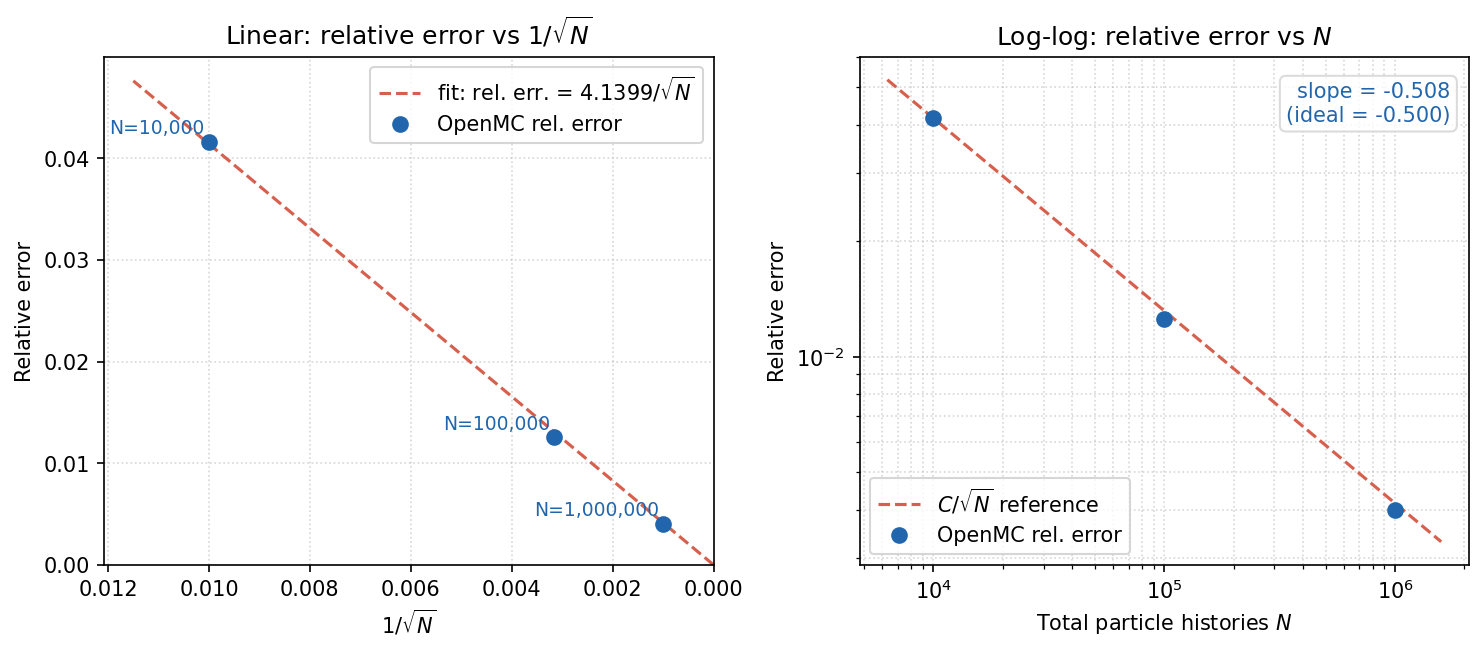
\includegraphics[width=0.95\textwidth]{../fundamental_testing/7221_se/7221_se_1.png} 
	\caption{Statistical convergence of results as a function of increasing simulated particle histories.} 
	\label{fig:7221-1} 
\end{figure}

\subsubsection{7.2.2.2 Test of statistical error with weight window}

Purpose: To verify the trend and correctness of statistical error with/without weight
window variance reduction techniques.

Test case: The models of the variance reduction examples.
Test method:Perform several independent calculations with increasing particle
histories 10,000, 100,000 and 1,000,000 with and without use of the variance reduction
technique(s). Then compare the trend of the statistical errors, check whether the
statistical error with variance reduction on is smaller than that without use of the VR
technique at the same histories. When calculating with a weight window, the variance
of the variance should be calculated, to verify the convergence of the calculation
results. Only results with the expected behaviour of the mean, variance, and the
variance of the sample variance should be considered valid for the statistical error test.

Problem was setup as described in and ran with OpenMC. The model is a simple concrete cube (2 m sides) with a 14 MeV neutron source. 
The qunatites of interst are tallies in cells at increasing shield thicknesses in 10 cm increments. The Random-Ray solver is used to create FW-CADIS based weight windows on the fly. Results:
\begin{figure}[H] 
	\centering 
	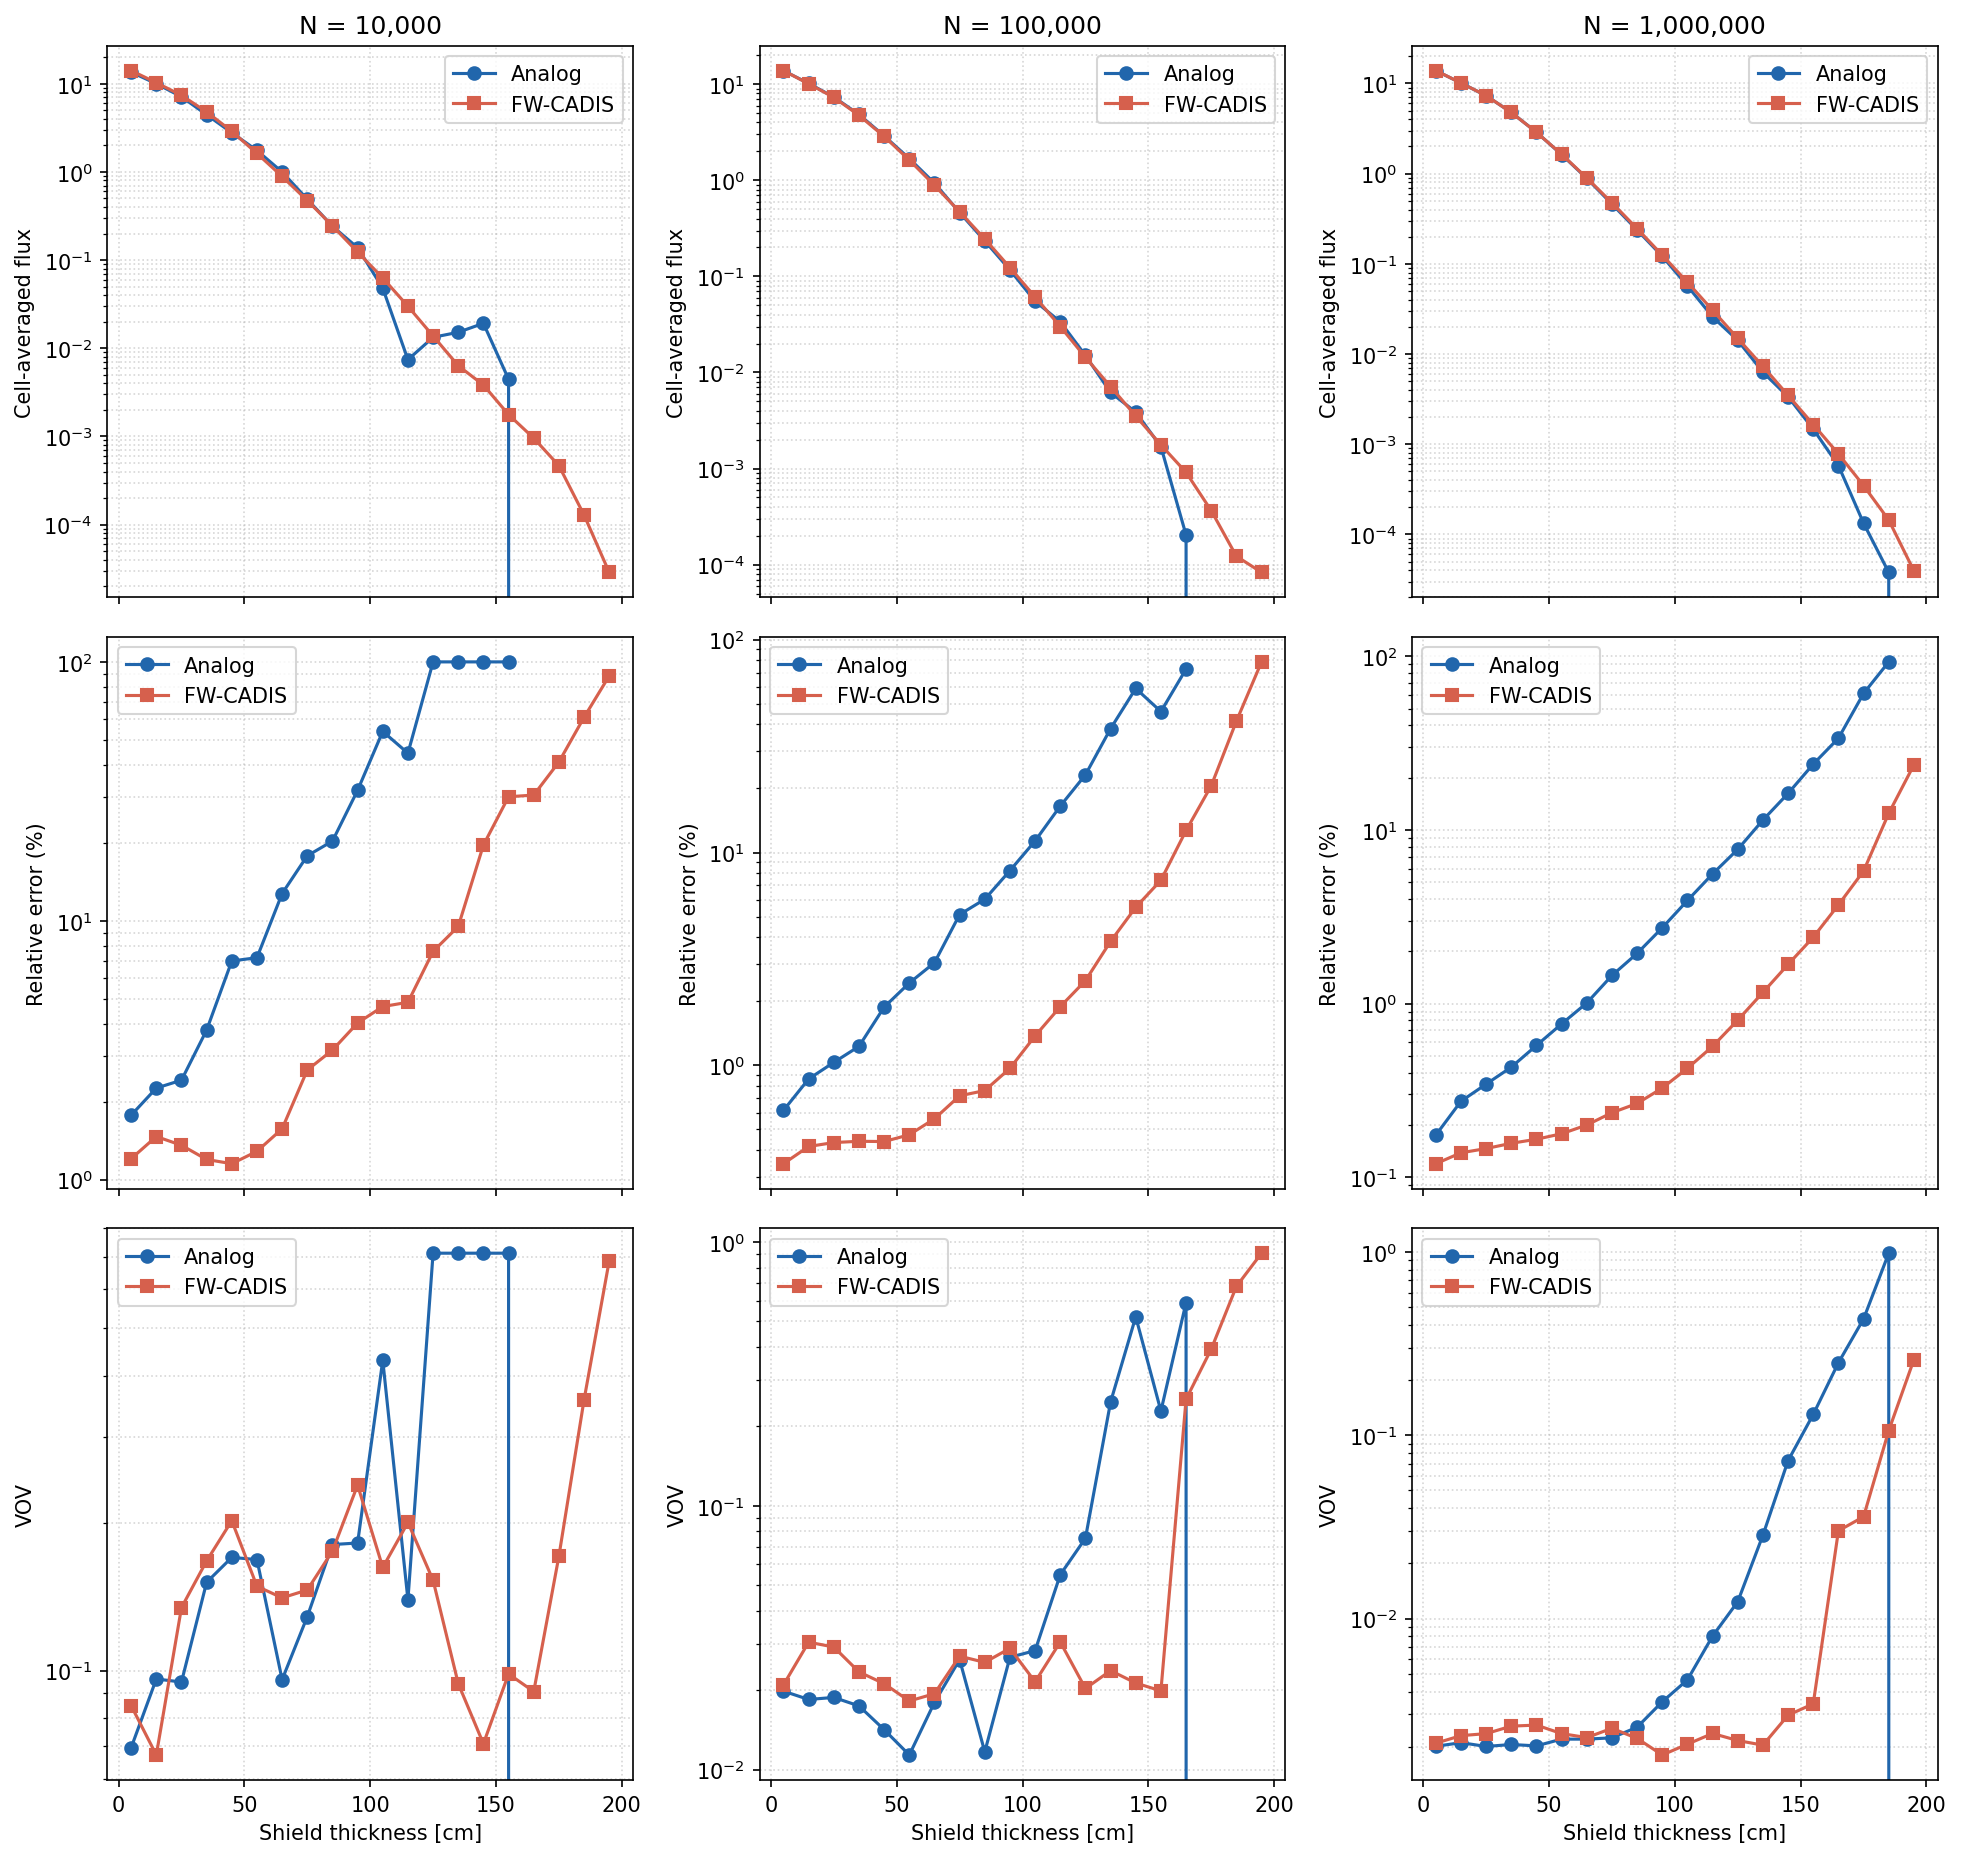
\includegraphics[width=0.95\textwidth]{../fundamental_testing/7222_seww/7222_seww_1.png} 
	\caption{Comparisson of analog and weight window accelerated simulation result as a function of shield thickness. Each colum represent a 10-fold increase in simulated particle histories.  Top row mean results, middle row relative error, bottom row Variance of Variance.} 
	\label{fig:7222-1} 
\end{figure}

\subsubsection{7.2.2.3 Test of random number generator}
Purpose: To verify the correctness of the random number generator. As random
number generators in Monte Carlo codes are implemented based on LCGs, this test is
aiming to verify the correctness of the LCGs implemented in the code.

Test case 1: The standard statistical tests for random number generators described by
Knuth or variations on Knuth's statistical tests.

The problem was setup as described. The random number generator was accessed via the DLL. A series of tests were run including:
Frequency, Serial, Runs, Gap, Poker, Autocorrelation.
For more details you can look at the full test report in: \path{/fundamental_testing/7223_rng/1} of the
\href{https://github.com/openmc-dev/openmc-fundamental-testing}{OpenMC Fundamental Testing git repository}.
\vspace{0.5em}
Test case 2: Marsaglia's DIEHARD test suite for random number generators.

Test Method: Write random stream generating program based on the LCGs code
implemented in the code. Apply the two test cases to the random stream generated by
the random stream generating program, if it passes the acceptance criteria, the random
number generator of the code can be considered as acceptable.

The problem was setup as described. The random number generator was accessed via the DLL. The Diehard test suite was run using the the modern implementation as part of Dieharder.
Diharder can be installed from the \href{https://github.com/seehuhn/dieharder}{Dieharder git repository} or in Ubuntu/Debian simply by \verb|sudo apt-get install dieharder|.

List of tests performed:
\begin{itemize} 
\item Birthday Spacings Test -- \verb|-d 0| (Diehard Birthdays Test) 
\item Binary Rank 31x31 and 32x32 -- \verb|-d 2| (Diehard 32x32 Binary Rank Test)
\item Binary Rank 6x8 -- \verb|-d 3| (Diehard 6x8 Binary Rank Test)
\item Bitstream -- \verb|-d 4| (Diehard Bitstream Test) 
\item OPSO (Overlapping-Pairs-Sparse-Occupancy) -- \verb|-d 5| (Diehard OPSO Test) 
\item OQSO (Overlapping-Quadruples-Sparse-Occupancy) -- \verb|-d 6| (Diehard OQSO Test) 
\item DNA -- \verb|-d 7| (Diehard DNA Test) 
\item Count the 1s (stream of bits) -- \verb|-d 8| (Diehard Count the 1s Stream Test) 
\item Count the 1s (specific byte) -- \verb|-d 9| (Diehard Count the 1s Byte Test) 
\item Parking Lot Test -- \verb|-d 10| (Diehard Parking Lot Test) 
\item Minimum Distance (2D circles/spheres) -- \verb|-d 11| (Diehard Minimum Distance Test) 
\item 3D Spheres (Minimum Distance) -- \verb|-d 12| (Diehard 3D Sphere Test) 
\item Squeeze Test -- \verb|-d 13| (Diehard Squeeze Test) 
\item Runs Test (Wald-Wolfowitz) -- \verb|-d 15| (Diehard Runs Test) 
\item Craps Test -- \verb|-d 16| (Diehard Craps Test) 
\end{itemize}

For more details you can look at the full test report in: \path{/fundamental_testing/7223_rng/2} of the
\href{https://github.com/seehuhn/dieharder}{OpenMC Fundamental Testing git repository}.

\subsubsection{7.2.2.4 Test of source sampling}
Purpose: To verify the correctness of the source sampling with probability distribution.

Test case 1: The model is a simple vacuum sphere with radius 5 cm, and the isotropic
neutron source is defined in the centre of the sphere with specific energy distribution.
Tally the neutron energy integrated over the sphere surface with refined energy bins.

Test method 1: Perform calculation until the tally results in each energy bin converge.
Compare the calculation results with the specific energy distribution of the source
definition, consider the code passes this test if the results meet the requirements
described in section 7.3.

Problem was setup as described and ran with OpenMC. A triangular enerrgy distibtuion was chosen. Results:
\begin{figure}[H] 
	\centering 
	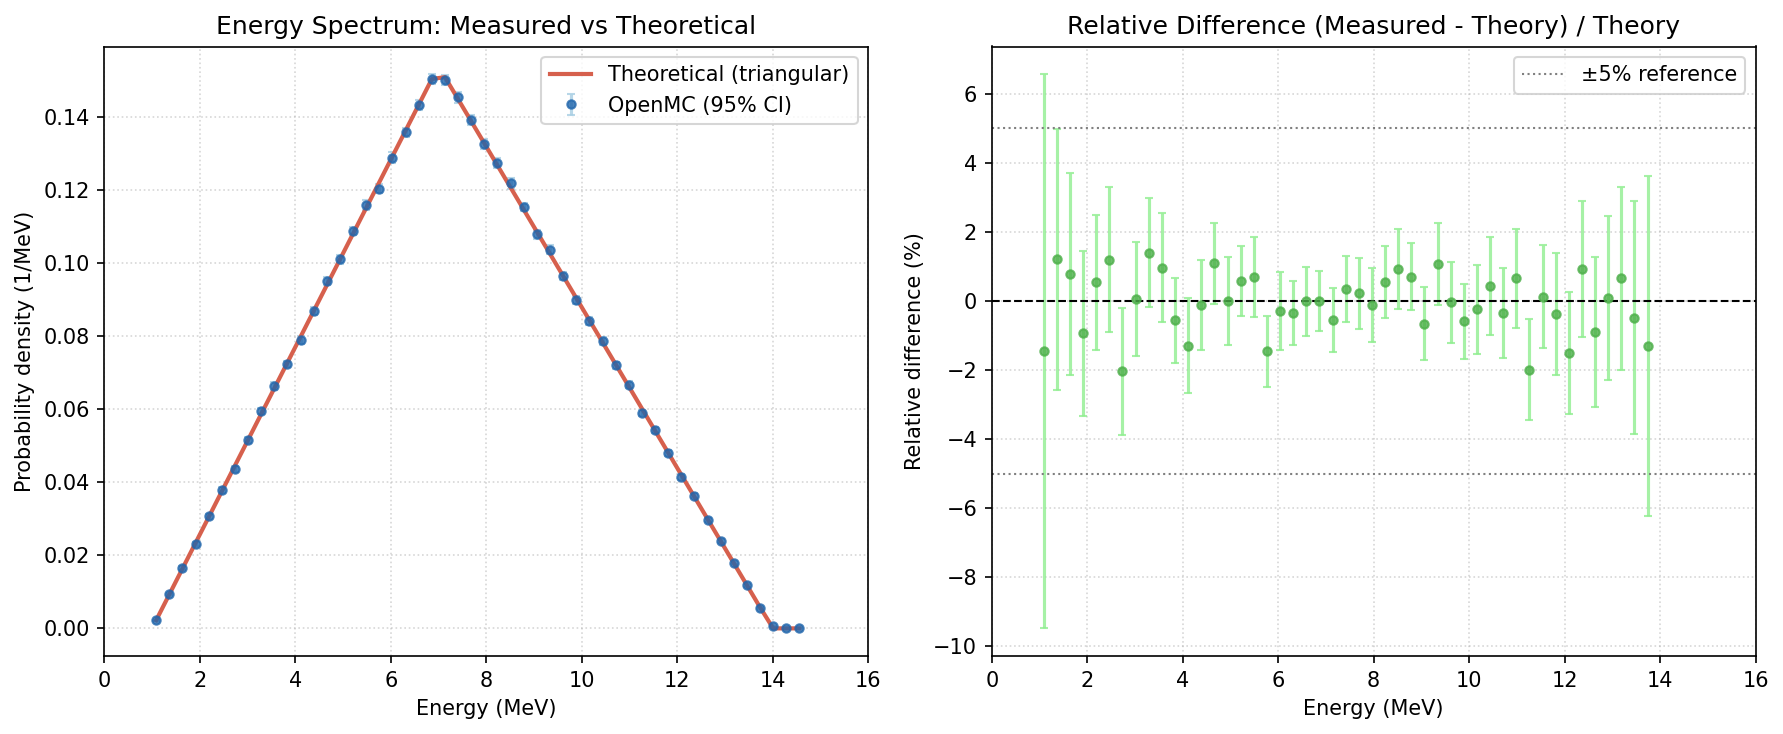
\includegraphics[width=0.95\textwidth]{../fundamental_testing/7224_ss/1/7224_ss_1.png} 
	\caption{Simulated vs theoretical source energy distribution.} 
	\label{fig:7224-1} 
\end{figure}
\vspace{0.5em}
Test case 2: The model is a simple vacuum cuboid pipe with length 10 cm*0.1 cm*0.1
cm (the coordinate of centre point is zero, dimension is defined in the order of x, y, z
axis). The neutron source is defined inside the plate with single direction along the z
axis, and the distribution of the source position is sampled by a specific distribution
along x axis and constant along y and z axis. The surface current of the top surface
(perpendicular to z axis and on the top of the cuboid pipe) segmented evenly to 100
segments by refined surfaces perpendicular to x axis are counted.

Test method 2: Perform calculations until all the tallies in all the segments converge.
Compare the results to the source position sampling, the code would be considered
passed this test if the results meet the criterial described in section 7.3.

Problem was setup as described and ran with OpenMC. A triangular positional distibtuion was chosen. Results:
\begin{figure}[H] 
	\centering 
	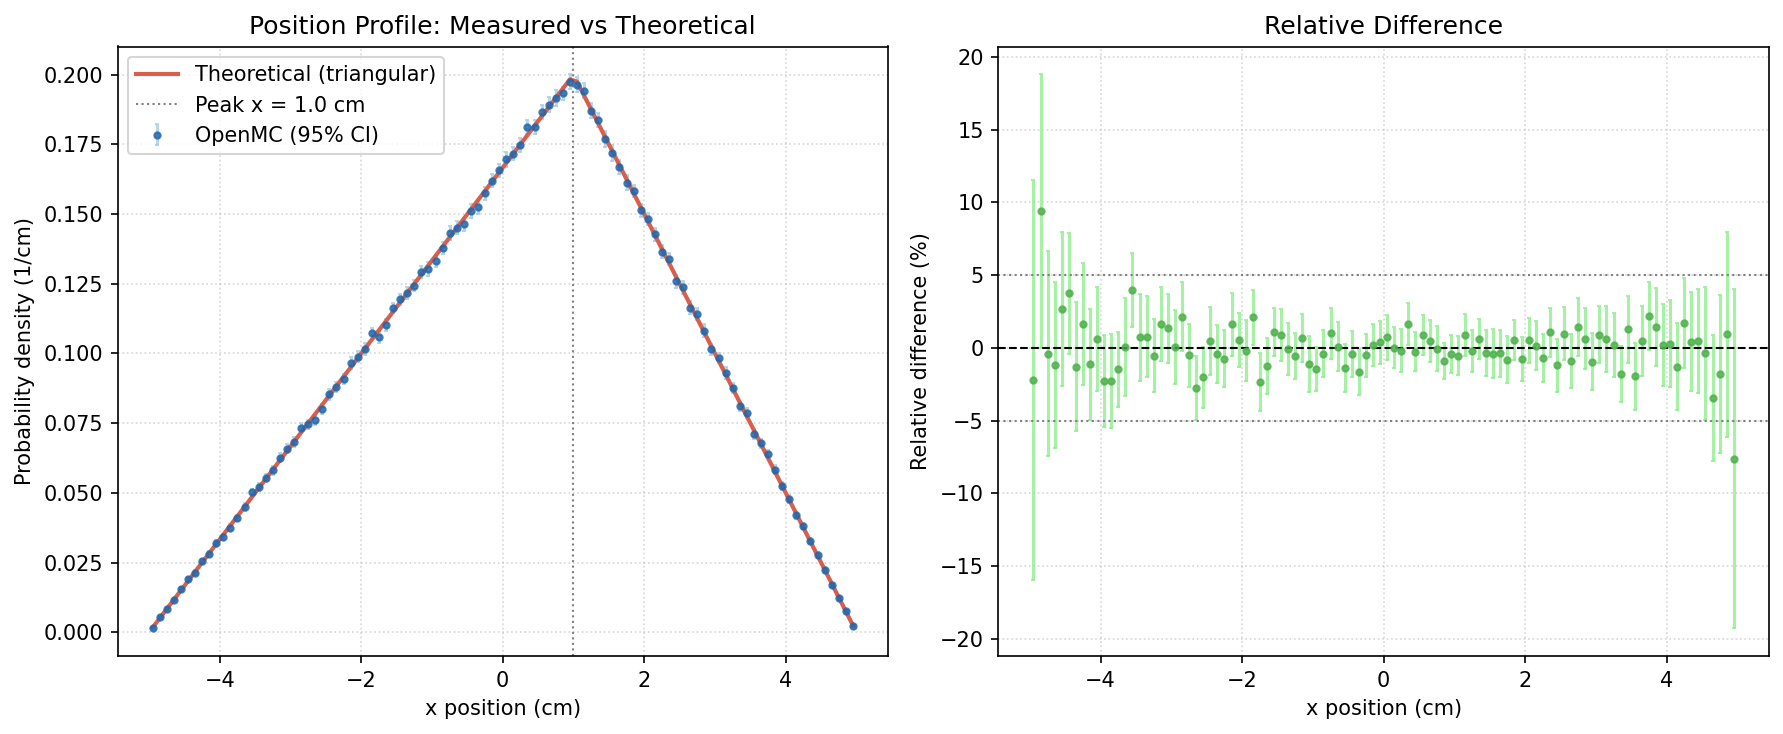
\includegraphics[width=0.95\textwidth]{../fundamental_testing/7224_ss/2/7224_ss_2.png} 
	\caption{Simulated vs theoretical source positional distribution.} 
	\label{fig:7224-2} 
\end{figure}

\vspace{0.5em}
Test case 3: The model is a simple vacuum circular slab with 5 cm radius and 1 cm
thickness along with z axis, and the mono neutron source (14MeV) is defined in the
centre line of the slab with specific direction distribution (perpendicular to z axis with
refined distributions). Split the slab into 365 segments that each segment is reference to
1 degree, and tally the neutron flux in each segment.

Test method 3: Perform calculations until all the tallies in all the source bins converge.
Compare he results to the source direction sampling, the code would be considered
passed that this test if the results met the criterial described in section 7.3.

Problem was setup as described and ran with OpenMC. A sinusioidal non-uniform azimuthal distribution angular distibtuion was chosen. Results:
\begin{figure}[H] 
	\centering 
	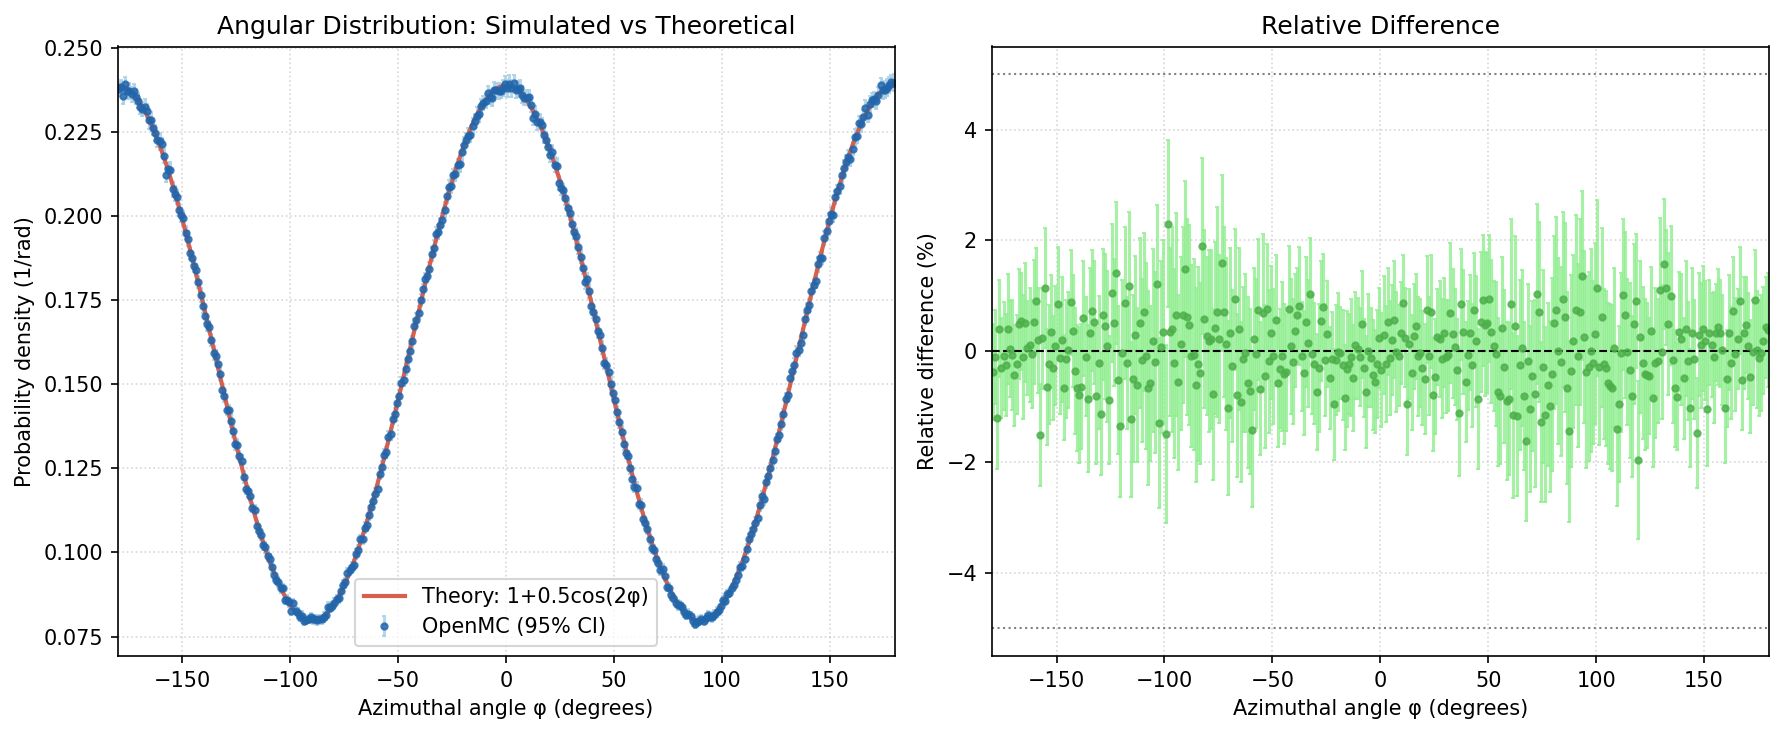
\includegraphics[width=0.95\textwidth]{../fundamental_testing/7224_ss/3/7224_ss_3.png} 
	\caption{Simulated vs theoretical source angular distribution.} 
	\label{fig:7224-3} 
\end{figure}

\vspace{0.5em}
Test case 4and the plasma solid with reflection surfaces is used as the test model. The
neutron flux in the mesh with grid size of 10cm*10cm*10cm covering the C-lite model
would be tallied.

Test method 4: Perform calculations until tallies of all the grids converge, compare the
results with MCNP results, considered the code passed this test if the results meet the
criteria described in section 7.3.

Problem was setup in MCNP and OpenMC according to the description. The ITER C-model plasma source was translated into OpenMC. Both the MCNP and OpenMC plasma source were postioned in to a voided wedge with reflective boundaried. Results:
\begin{figure}[H] 
	\centering 
	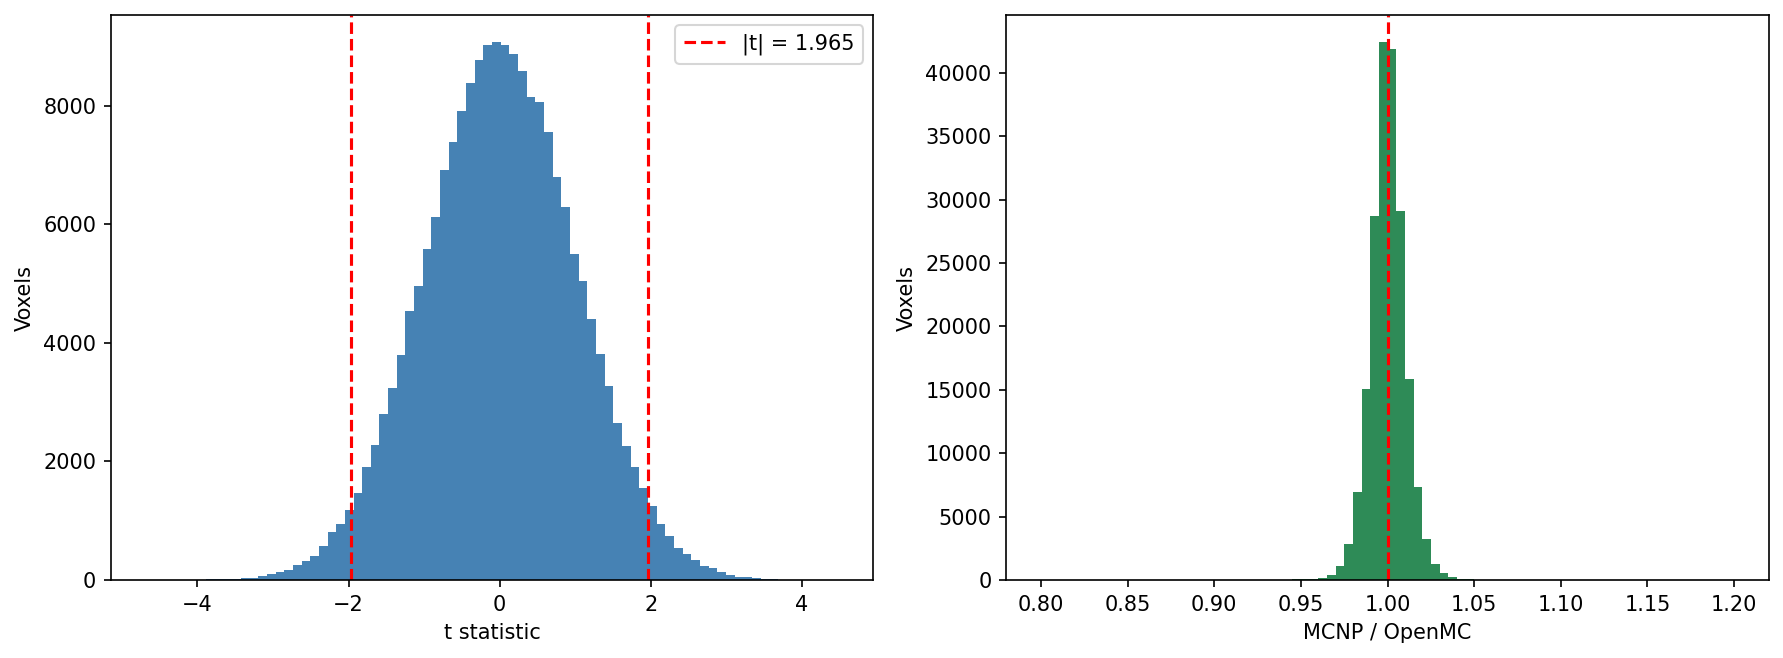
\includegraphics[width=0.95\textwidth]{../fundamental_testing/7224_ss/4/7224_ss_4-TTest.png} 
	\caption{Student t-statisitical test results and ratio of fluxes on a 10cm mesh in MCNP and OpenMC.} 
	\label{fig:7224-4} 
\end{figure}

\begin{figure}[H] 
	\centering 
	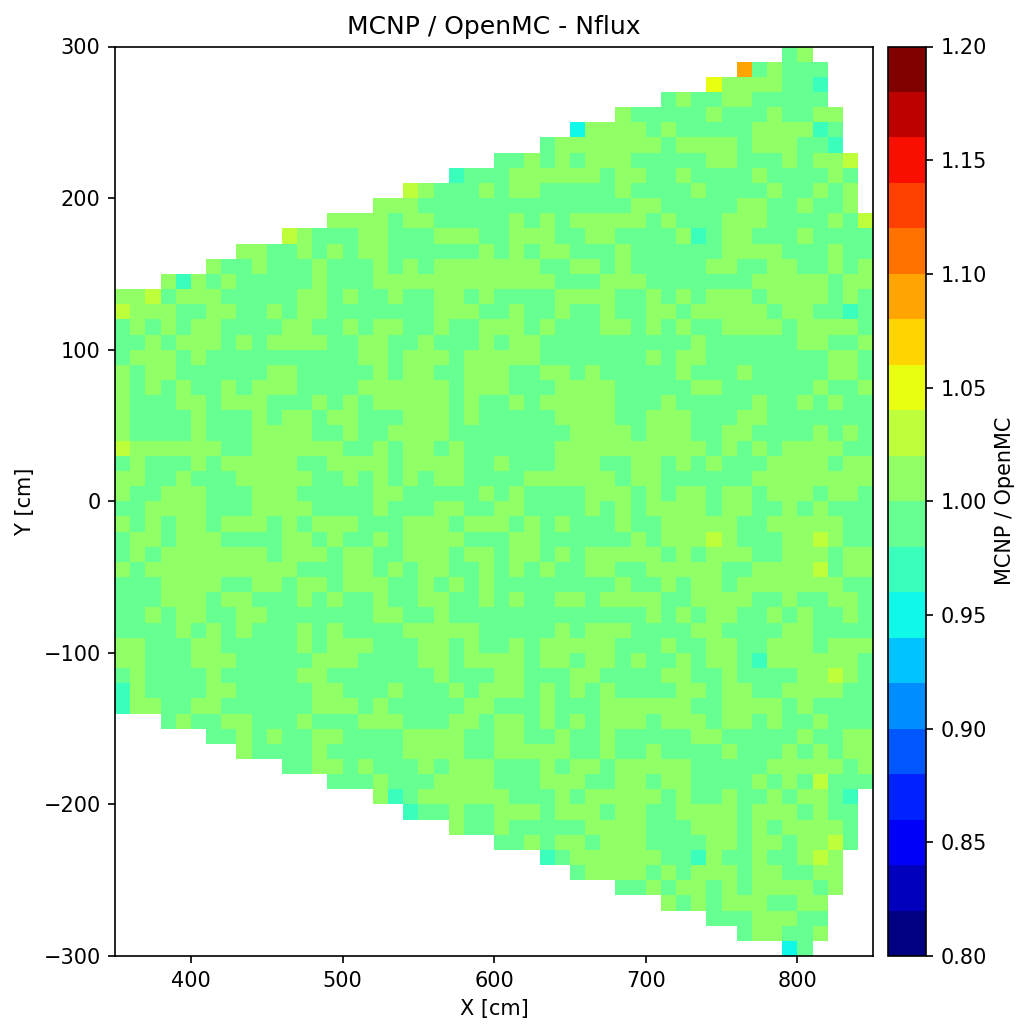
\includegraphics[width=0.54\textwidth]{../fundamental_testing/7224_ss/4/7224_ss_4-Ratio_XY_.png} 
	\hfill 
	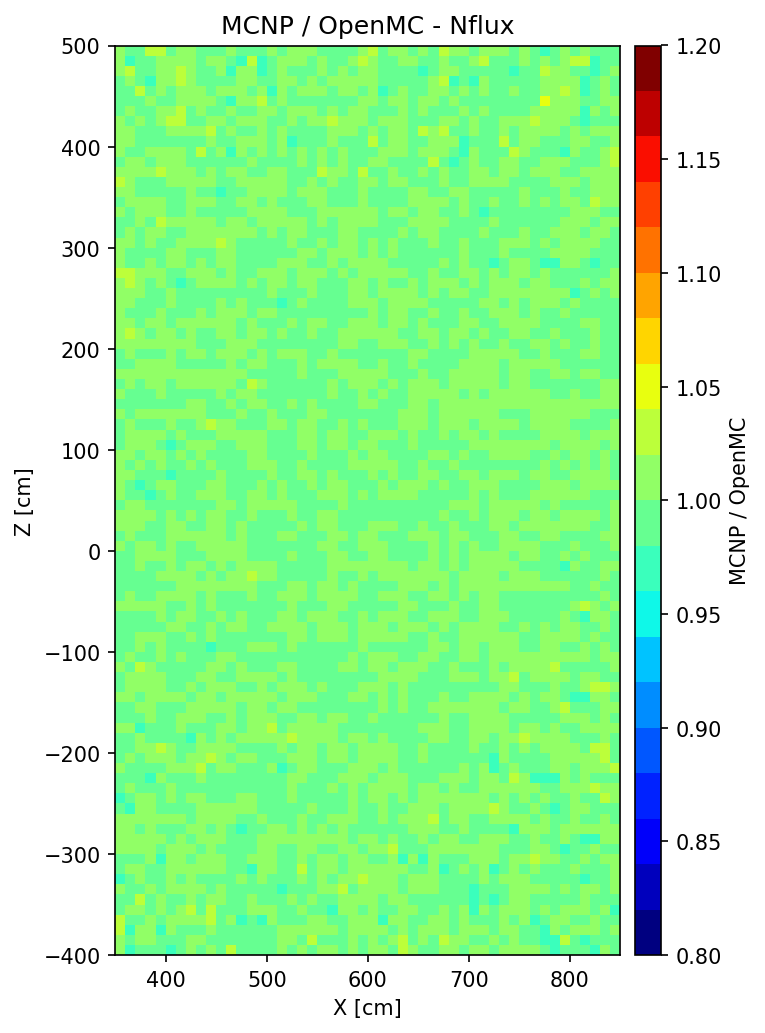
\includegraphics[width=0.44\textwidth]{../fundamental_testing/7224_ss/4/7224_ss_4-Ratio_XZ_.png} 
	\caption{Ratio of MCNP and OpenMC neutron flux over plasma source with reflective boundaries. XY plane (left), XZ plane (right).} 
	\label{fig:7224-4-ratios} 
\end{figure}

\subsubsection{7.2.2.5 Test of conservation of energy for nuclear reaction}
Purpose: To verify the correctness of energy conservation for nuclear reaction.

Test case: The model is a cuboid (50 cm*50 cm*50 cm) with nature iron. The
neutron source is located in the bottom of the cuboid with direction to the negative half
of z axis and mono energy 14MeV. The neutron and photon energy integrated over each
surface of cuboid are counted, as well as heating inside the cuboid.

Test method: Perform the calculation with 100,000,000 particles, and count the
entered and leakage neutron and photon energy independently.

Compare the entered neutron energy A, nuclear heat deposition of neutron and photon
B and the leakage of neutron and photon energy C, then get the subtraction (B+C-A).
The next step, the comparison should be done between the subtraction value and the (n,gamma) 
reaction deposition energy calculated by the code, consider the code passes this test if
the reaction deposition energy has been included in the subtraction value.
\vspace{0.5em}
Problem was setup as described and ran with OpenMC. However the wording of the test is ambigious. It is hard to prove quote: \textit{if the reaction deposition energy has been included in the subtraction value} at the specified 
14 MeV where several reaction (including thresholed) reactions occur that staurate the overall \textit{subtraction value} as it is seen in Figure \ref{fig:7225-1}.
\begin{figure}[H] 
	\centering 
	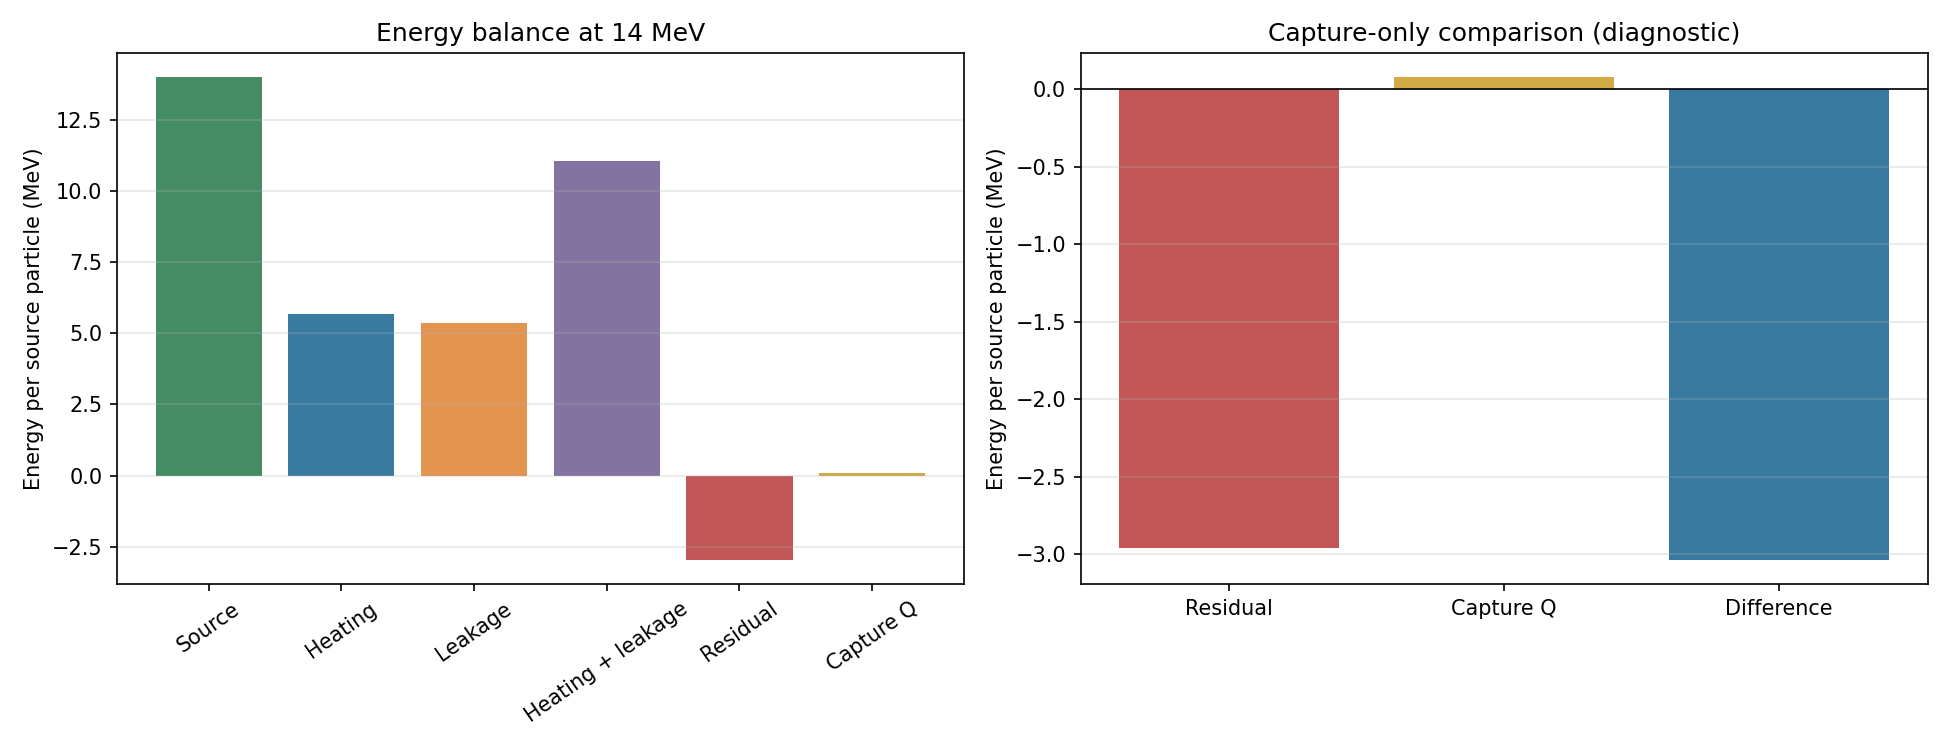
\includegraphics[width=0.95\textwidth]{../fundamental_testing/7225_ce/1/7225_ce_1.png} 
	\caption{Enerergy balance with 14 MeV neutron source. A large residual energy is observed which can be attributed to several reaction channels such as: (n,2n), (n,p), (n,alpha)} 
	\label{fig:7225-1} 
\end{figure}

We propose to ammend the test and run it with 1 MeV neutrons where the energy balance is much simpler and where indeed the subtraction value is close to the capture reaction deposition energy. Results with the 1 MeV source is shown in Figure \ref{fig:7225-2}.  Both tests are performed, but the Summary Results table \ref{tab:fund_res} is linked to the 1 MeV case.
\begin{figure}[H] 
	\centering 
	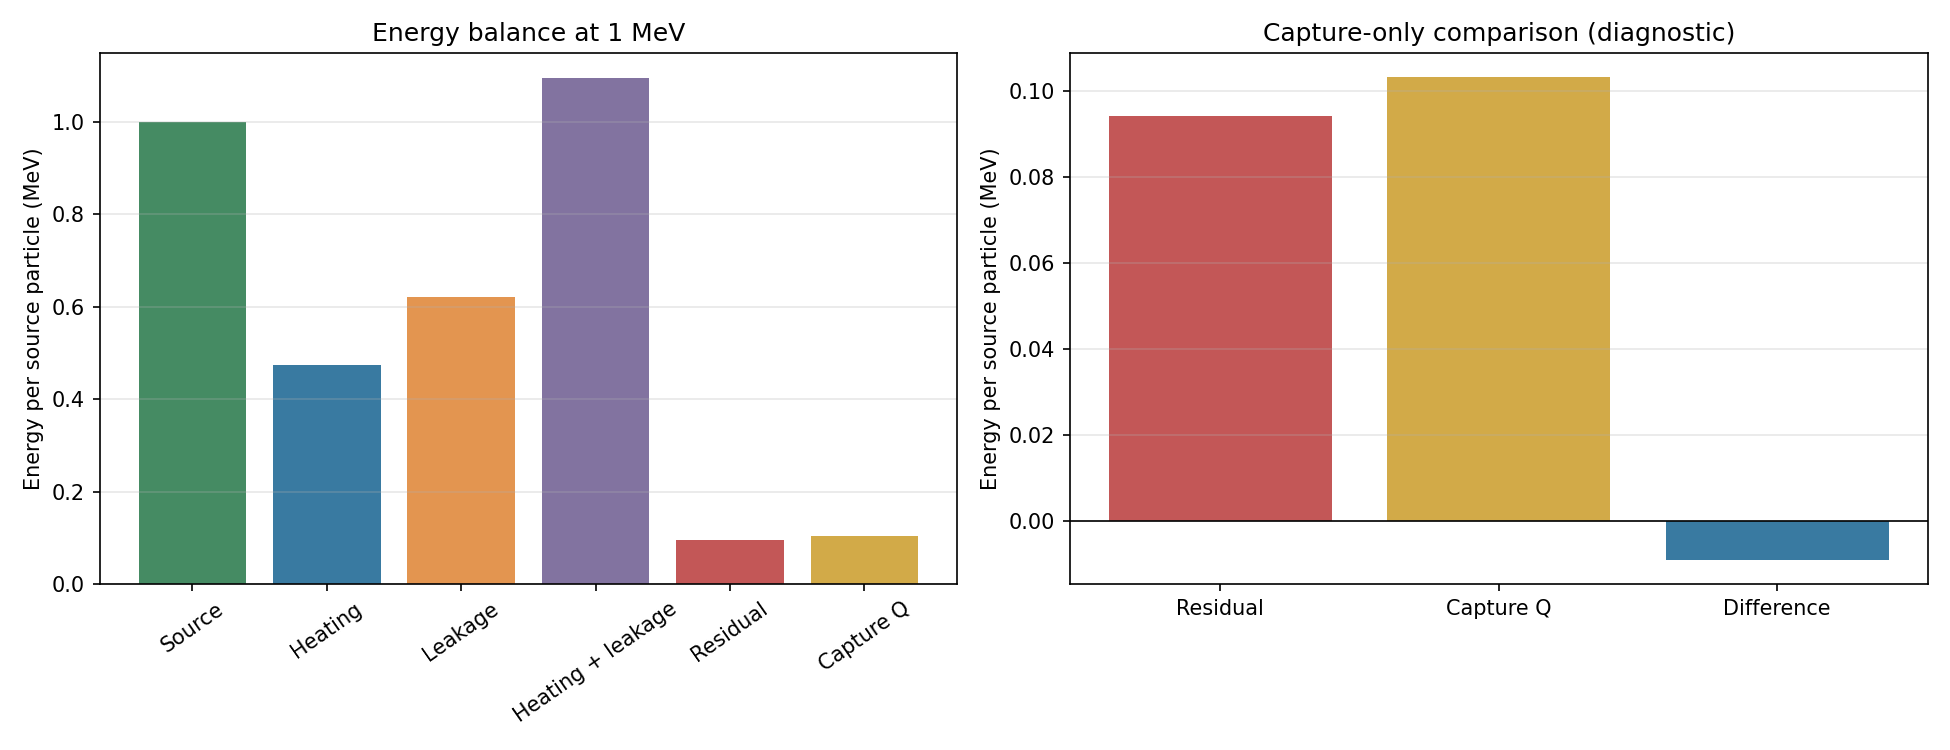
\includegraphics[width=0.95\textwidth]{../fundamental_testing/7225_ce/2/7225_ce_2.png} 
	\caption{Enerergy balance with 14 MeV neutron source. The residual is within uncertainty of the caputre reaction energy depostion.} 
	\label{fig:7225-2} 
\end{figure}



\newpage

\section{Quick Install Guide}
\label{quickinstall}

This quick install guide outlines the basic steps needed to install OpenMC on
your computer. For more detailed instructions on configuring and installing
OpenMC, see the User's Manual.

\subsection*{Installing on Linux/Mac with Conda}

\href{https://docs.conda.io/en/latest/}{Conda} is an open source package management
system and environments management system for installing multiple versions of
software packages and their dependencies and switching easily between them.
OpenMC can be installed in a \texttt{conda} environment. First, \texttt{conda} should be
installed (\href{https://www.anaconda.com/docs/getting-started/getting-started}{installation guide})
with either Anaconda Distribution or Miniconda. Once you have \texttt{conda} installed
on your system, OpenMC can be installed via the \texttt{conda-forge} channel.

First, add the \texttt{conda-forge} channel with:

\begin{verbatim}
conda config --add channels conda-forge
conda config --set channel_priority strict
\end{verbatim}

Then create and activate a new conda environment called \texttt{openmc-env} (or whatever
you wish) with OpenMC installed.

\begin{verbatim}
conda create --name openmc-env openmc
conda activate openmc-env
\end{verbatim}

If you are installing on macOS with an Apple silicon ARM-based processor, you
will also need to specify the \texttt{--platform} option:

\begin{verbatim}
conda create --name openmc-env --platform osx-64 openmc
\end{verbatim}

You are now in a conda environment called \texttt{openmc-env} that has OpenMC installed.

\subsection*{Installing on Linux/Mac/Windows with Docker}

OpenMC can be easily deployed using \href{https://www.docker.com/}{Docker} on any
Windows, Mac, or Linux system. With Docker running, execute the following command
in the shell to download and run a Docker image with the most recent release
of OpenMC from \href{https://hub.docker.com/}{DockerHub}:

\begin{verbatim}
docker run openmc/openmc:latest
\end{verbatim}

This will take several minutes to run depending on your internet download speed.
The command will place you in an interactive shell running in a Docker
container with OpenMC installed.

\paragraph{Note}
The \texttt{docker run} command supports many \href{https://docs.docker.com/engine/reference/commandline/run/}{options}
for spawning containers including \href{https://docs.docker.com/storage/volumes/}{mounting volumes}
from the host filesystem, which many users will find useful.

\subsection*{Installing from Source using Spack}

\href{https://spack.readthedocs.io/en/latest/}{Spack} is a package management tool designed to support multiple versions and
configurations of software on a wide variety of platforms and environments.
Please follow Spack's \href{https://spack.readthedocs.io/en/latest/getting_started.html}{setup guide} to configure the system.

To install the latest OpenMC with the Python API, use the following command:

\begin{verbatim}
spack install py-openmc
\end{verbatim}

For more information about customizations including MPI, see the detailed installation
instructions using Spack. Once installed, environment/lmod modules can be generated
or Spack's \texttt{load} feature can be used to access the installed packages.

\subsection*{Manually Installing from Source}

\subsubsection*{Obtaining prerequisites on Ubuntu}

When building OpenMC from source, all prerequisites can
be installed using the package manager:

\begin{verbatim}
sudo apt install g++ cmake libhdf5-dev libpng-dev
\end{verbatim}

After the packages have been installed, follow the instructions to build from source below.

\subsubsection*{Obtaining prerequisites on macOS}

For an OpenMC build with multithreading enabled, a package manager like
\href{https://brew.sh}{Homebrew} should first be installed. Then, the following
packages should be installed, for example in Homebrew via:

\begin{verbatim}
brew install llvm cmake xtensor hdf5 python libomp libpng
\end{verbatim}

The compiler provided by the above LLVM package should be used in place of the
one provisioned by XCode, which does not support the multithreading library used
by OpenMC. To ensure CMake picks up the correct compiler, make sure that either
the \texttt{CXX} environment variable is set to the brew-installed \texttt{clang++}
or that the directory containing it is on your \texttt{PATH} environment
variable. Common locations for the brew-installed compiler are
\texttt{/opt/homebrew/opt/llvm/bin} and \texttt{/usr/local/opt/llvm/bin}.

After the packages have been installed, follow the instructions to build from
source below.

\subsection*{Building Source on Linux or macOS}

All OpenMC source code is hosted on \href{https://github.com/openmc-dev/openmc}{GitHub}.
If you have \href{https://git-scm.com}{git}, a modern C++ compiler,
\href{https://cmake.org}{CMake}, and \href{https://www.hdfgroup.org/solutions/hdf5/}{HDF5}
installed, you can download and install OpenMC by entering the following commands
in a terminal:

\begin{verbatim}
git clone --recurse-submodules https://github.com/openmc-dev/openmc.git
cd openmc
mkdir build && cd build
cmake ..
make
sudo make install
\end{verbatim}

This will build an executable named \texttt{openmc} and install it (by default in
\texttt{/usr/local/bin}). If you do not have administrator privileges, the cmake command
should specify an installation directory where you have write access, e.g.

\begin{verbatim}
cmake -DCMAKE_INSTALL_PREFIX=$HOME/.local ..
\end{verbatim}

The \texttt{openmc} Python package must be installed separately. The easiest way
to install it is using \href{https://pip.pypa.io/en/stable/}{pip}.
From the root directory of the OpenMC repository, run:

\begin{verbatim}
python -m pip install .
\end{verbatim}

By default, OpenMC will be built with multithreading support. To build
distributed-memory parallel versions of OpenMC using MPI or to configure other
options, directions can be found in the detailed installation instructions.

\newpage
\section{What's New in 0.15.3}

\subsection*{Summary}

This release of OpenMC includes many bug fixes, performance improvements, and
several notable new features. The major highlights of this release include a new
\texttt{openmc.deplete.R2SManager} class that automates the workflow for
rigorous 2-step (R2S) shutdown dose rate calculations, the ability to collect
higher moments for tally results that can be used to test normality, a new
uncertainty-aware criticality search method, a new collision tracking feature
that enables detailed tracking of particle interactions, support for distributed
cell densities, and several new tally filters. The random ray solver also
continues to receive significant updates, including automatic setup
capabilities, improved geometry handling, and better weight window support.
Depletion capabilities have been expanded with thermochemical redox control,
external transfer rates, and improved performance.

\subsection*{Compatibility Notes and Deprecations}

MCPL has been changed from a build-time dependency to a runtime optional
dependency, which means OpenMC will attempt to load the MCPL library at
runtime when needed rather than requiring it at build time.

The \texttt{openmc.mgxs.Library.add\_to\_tallies\_file} method has been renamed to\newline
\texttt{openmc.mgxs.Library.add\_to\_tallies}.

\subsection*{New Features}

\begin{itemize}
\item A new collision tracking feature enables detailed tracking of particle interactions (\href{https://github.com/openmc-dev/openmc/pull/3417}{\#3417})
\item Added \texttt{openmc.model.Model.keff\_search} method for automated criticality searches (\href{https://github.com/openmc-dev/openmc/pull/3569}{\#3569})
\item Introduced automated workflow for mesh- or cell-based R2S calculations (\href{https://github.com/openmc-dev/openmc/pull/3508}{\#3508})
\item Ability to source electron/positrons directly for charged particle simulations (\href{https://github.com/openmc-dev/openmc/pull/3404}{\#3404})
\item Multi-group capability for kinetics parameter calculations with Iterated Fission Probability (\href{https://github.com/openmc-dev/openmc/pull/3425}{\#3425})
\item Introduced a new \texttt{openmc.MeshMaterialFilter} class (\href{https://github.com/openmc-dev/openmc/pull/3406}{\#3406})
\item Added support for distributed cell densities (\href{https://github.com/openmc-dev/openmc/pull/3546}{\#3546})
\item Implemented a \texttt{openmc.WeightWindowsList} class that enables export to HDF5 (\href{https://github.com/openmc-dev/openmc/pull/3456}{\#3456})
\item Added \texttt{openmc.Material.mean\_free\_path} method (\href{https://github.com/openmc-dev/openmc/pull/3469}{\#3469})
\item Introduced \texttt{openmc.lib.TemporarySession} context manager (\href{https://github.com/openmc-dev/openmc/pull/3475}{\#3475})
\item Added material depletion function for tracking individual material depletion (\href{https://github.com/openmc-dev/openmc/pull/3420}{\#3420})
\item Added methods on \texttt{openmc.Material} class for waste disposal rating/classification (\href{https://github.com/openmc-dev/openmc/pull/3366}{\#3366}, \href{https://github.com/openmc-dev/openmc/pull/3376}{\#3376})
\item Support for thermochemical redox control transfer rates in depletion (\href{https://github.com/openmc-dev/openmc/pull/2783}{\#2783})
\item Support for external transfer rates source term in depletion (\href{https://github.com/openmc-dev/openmc/pull/3088}{\#3088})
\item Added combing capability for fission site sampling and delayed neutron emission time (\href{https://github.com/openmc-dev/openmc/pull/2992}{\#2992})
\item Ability to specify reference direction for azimuthal angle in \texttt{openmc.stats.PolarAzimuthal} distribution (\href{https://github.com/openmc-dev/openmc/pull/3582}{\#3582})
\item Allow spatial constraints on element sources within \texttt{openmc.MeshSource} (\href{https://github.com/openmc-dev/openmc/pull/3431}{\#3431})
\item Added VTK HDF (.vtkhdf) format support for writing VTK data (\href{https://github.com/openmc-dev/openmc/pull/3252}{\#3252})
\item Implemented filter weight capability (\href{https://github.com/openmc-dev/openmc/pull/3345}{\#3345})
\item Optionally collect higher moments for tallies (\href{https://github.com/openmc-dev/openmc/pull/3363}{\#3363})
\end{itemize}

\paragraph{Random Ray Solver Enhancements}
\begin{itemize}
\item Random Ray AutoMagic Setup for automatic configuration (\#3351)
\item Point source locator for random ray mode (\#3360)
\item Support for DAGMC geometries (\#3374)
\item Optimized mapping of source regions to tallies (\#3465)
\item Base source region refactor (\#3576)
\end{itemize}

\subsection*{Bug Fixes and Small Changes}

\begin{itemize}
\item Add two MPI barriers in R2S workflow (\#3646)
\item Fix a few warnings, rename add\_to\_tallies\_file (\#3639)
\item Fix typo in DAGMC lost particle test (\#3634)
\item Avoid multiprocessing Pool when running depletion tests with MPI (\#3633)
\item Support MPI parallelism in R2SManager (\#3632)
\item Update documentation for particle tracks (\#3627)
\item Adding variance of variance and normality tests for tally statistics (\#3454)
\item Avoid divide-by-zero in \texttt{from\_multigroup\_flux} when flux is zero (\#3624)
\item Write particle states as separate lines in track VTK files (\#3628)
\item Reset DAGMC history when reviving from source (\#3601)
\item Add energy group structure: SCALE-999 (\#3564)
\item Fix bug in normalization of tally results with no\_reduce (\#3619)
\item Enable nuclide filters with get\_decay\_photon\_energy (\#3614)
\item Update \texttt{check\_type} calls to accept both \texttt{str} and \texttt{os.PathLike} objects (\#3618)
\item Speed up \texttt{apply\_time\_correction} by reducing file I/O and deepcopies (\#3617)
\item FW-CADIS Disregard Max Realizations Setting (\#3616)
\item Random Ray Geometry Debug Mode Fix (\#3615)
\item Don't write reaction rates in depletion results by default (\#3609)
\item Allow Path objects in MGXSLibrary.export\_to\_hdf5 (\#3608)
\item Clip mixture distributions based on mean times integral (\#3603)
\item Allow V0 in atomic\_mass function (\#3607)
\item Re-run flaky tests when needed (\#3604)
\item Ability to load mesh objects from weight\_windows.h5 file (\#3598)
\item Switch to using coveralls github action for reporting (\#3594)
\item Add user setting for free gas threshold (\#3593)
\item Speed up time correction factors (\#3592)
\item Fix caching issue when using NCrystal materials (\#3538)
\item Fix random ray source region mesh export (\#3579)
\item Ensure weight\_windows\_file information is read from XML (\#3587)
\item Add missing documentation on \textless source\textgreater{} (\#3590)
\item Adding tally filter type option (\#3584)
\item Optional separation of mesh-material-volume calc (\#3581)
\item Fix IFP implementation (\#3580)
\item Remove several TODOs related to C++17 (\#3574)
\item Fix performance regression in libMesh tallies (\#3577)
\item Update find\_package calls (\#3572)
\item Ensure \texttt{n\_dimension\_} attribute is set (\#3575)
\item Allow newer Sphinx version (\#3571)
\item Fixed bug combining filters (\#3525)
\item PowerLaw negative interval error (\#3542)
\item Fix chain matrix performance (\#3567)
\item Do not apply boundary conditions in volume calc (\#3562)
\item Bump tolerance for activation test (\#3560)
\item Fixed cross-section plotting bug (\#3558)
\item Change test order (\#3533)
\item adding ecco 33 (\#3556)
\item Refactor endf\_data (\#3539)
\item Revert "fix broken CI" (\#3554)
\item fix broken CI (\#3551)
\item Leverage particle.move\_distance (\#3544)
\item fix tests broken (\#3543)
\item not printing 0 percent nuclides (\#3448)
\item Fix time cutoff bug (\#3526)
\item Avoid duplicate materials in XML (\#3536)
\item Use cached property for sources (\#3535)
\item better error message (\#3534)
\item Adding 616 group structure (\#3531)
\item Remove unused accessors (\#3527)
\item Consistent XML parsing (\#3517)
\item Add stat:sum field (\#3522)
\item Remove reorder\_attributes (\#3519)
\item Fix MeshMaterialFilter bug (\#3520)
\item Fix distribcell offsets (\#3424)
\item Add FW-CADIS DAGMC test (\#3504)
\item Fix Weight Window scaling (\#3511)
\item Fix list input bug (\#3513)
\item Allow initialized TemporarySession (\#3505)
\item Update DAGMC definitions (\#3510)
\item Avoid duplicate filters (\#3506)
\item Enable MCPL source files (\#3472)
\item Boundary accessors (\#3496)
\item Auto dimension for mesh (\#3468)
\item Add LocalCoord accessors (\#3494)
\item Make MCPL runtime optional (\#3429)
\item Use auto-chunking HDF5 (\#3498)
\item Get ID maps from Model (\#3481)
\item Update OSX install instructions (\#3501)
\item Update conda instructions (\#3488)
\item Only show warning in restart mode (\#3478)
\item Add CMake submodule flag (\#3480)
\item Added citation metadata file (\#3409)
\item fix zam parsing (\#3484)
\item Support flux collapse method (\#3466)
\item Stabilize Adjoint Source (\#3476)
\item Refactor Configuration Management (\#3461)
\item Updated Docs (\#3473)
\item Parallel Weight Window Update (\#3467)
\item Limit Random Ray Weight Window Generation (\#3464)
\item Fix Dockerfile DAGMC (\#3463)
\item Fix Weight Window loop bug (\#3457)
\item Weight Window Birth Scaling (\#3459)
\item geometry.plot fixes (\#3458)
\item Fix DAGMC plot crash (\#3455)
\item Fix Ta expansion bug (\#3443)
\item Prevent Adjoint Infinity (\#3449)
\item add DAGMC plot (\#3451)
\item Allow equiprobable angles (\#3346)
\item Change Docker base image (\#3442)
\item Fix MGXS IDs (\#3437)
\item Allow chain\_file as object (\#3436)
\item update flux units (\#3441)
\item Fix raytrace loop (\#3423)
\item Apply max events check (\#3438)
\item Source rejection fraction (\#3433)
\item Fix spherical mesh (\#3428)
\item Random Ray policy change (\#3434)
\item Plotting fix (\#3430)
\item Avoid negative heating (\#3426)
\item Fix serialization bug (\#3421)
\item Fix timestep start data (\#3414)
\item Fix charged particle deposition (\#3416)
\item Fix duplicate mesh XML (\#3418)
\item Debian typo (\#3411)
\item DAGMC plot test (\#3375)
\item Memory fixes (\#3405)
\item type hints (\#3399)
\item resolve paths (\#3400)
\item Fix CDF computation (\#3396)
\item Fix source weighting (\#3395)
\item VTK checks update (\#3371)
\item Map Compton data (\#3392)
\item Skip atomic relaxation (\#3391)
\item Fix large bremsstrahlung yields (\#3386)
\item Fix tally name (\#3383)
\item Install MCPL in CI (\#3388)
\item Chain level reduction (\#3377)
\item Fix CylindricalMesh distances (\#3370)
\item EnergyFilter bin check (\#3372)
\item Fix LLVM loading (\#3368)
\item Plot ID reporting (\#3361)
\item Handle missing tags (\#3359)
\item Add kg units (\#3358)
\end{itemize}

\newpage
\section{Publications}
\label{publications}

\subsection{Overviews}

\begin{itemize}
\item Paul K. Romano, Nicholas E. Horelik, Bryan R. Herman, Adam G. Nelson, Benoit
Forget, and Kord Smith, ``\href{https://doi.org/10.1016/j.anucene.2014.07.048}{OpenMC: A State-of-the-Art Monte Carlo Code for Research and Development},''
\textit{Ann. Nucl. Energy}, \textbf{82}, 90--97 (2015).

\item Paul K. Romano, Bryan R. Herman, Nicholas E. Horelik, Benoit Forget, Kord
Smith, and Andrew R. Siegel, ``Progress and Status of the OpenMC Monte Carlo
Code,'' \textit{Proc. Int. Conf. Mathematics and Computational Methods Applied to
Nuclear Science and Engineering}, Sun Valley, Idaho, May 5--9 (2013).

\item Paul K. Romano and Benoit Forget, ``\href{https://doi.org/10.1016/j.anucene.2012.06.040}{The OpenMC Monte Carlo Particle Transport Code},''
\textit{Ann. Nucl. Energy}, \textbf{51}, 274--281 (2013).
\end{itemize}

\subsection{Benchmarking}

\begin{itemize}
\item Travis J. Labossiere-Hickman and Benoit Forget, ``Selected VERA Core Physics
Benchmarks in OpenMC,'' \textit{Trans. Am. Nucl. Soc.}, \textbf{117}, 1520--1523 (2017).

\item Khurrum S. Chaudri and Sikander M. Mirza, ``\href{https://doi.org/10.1016/j.pnucene.2014.12.018}{Burnup dependent Monte Carlo neutron physics calculations of IAEA MTR benchmark},''
\textit{Prog. Nucl. Energy}, \textbf{81}, 43--52 (2015).

\item Daniel J. Kelly et al., ``Analysis of select BEAVRS PWR benchmark cycle 1 results using MC21 and OpenMC,'' \textit{Proc. PHYSOR}, Kyoto, Japan, Sep. 28--Oct. 3 (2014).

\item Bryan R. Herman et al., ``Analysis of tally correlations in large light water reactors,'' \textit{Proc. PHYSOR}, Kyoto, Japan, Sep. 28--Oct. 3 (2014).

\item Nicholas Horelik et al., ``Benchmark for Evaluation and Validation of Reactor Simulations,'' \textit{Proc. Int. Conf. Mathematics and Computational Methods Applied to Nuclear Science and Engineering}, Sun Valley, Idaho, May 5--9 (2013).

\item Jonathan A. Walsh et al., ``Validation of OpenMC Reactor Physics Simulations with the B\&W 1810 Series Benchmarks,'' \textit{Trans. Am. Nucl. Soc.}, \textbf{109}, 1301--1304 (2013).
\end{itemize}

\subsection{Coupling and Multi-physics}

\begin{itemize}
    
\item Miriam A. Kreher, Benoit Forget, and Kord Smith, ``Single-Batch Monte Carlo
Multiphysics Coupling,'' \textit{Proc. M\&C}, 1789--1797, Portland, Oregon, Aug.\ 25--29 (2019).

\item Ze-Long Zhao, Yongwei Yang, and Shuang Hong, ``Application of FLUKA and OpenMC
in coupled physics calculation of target and subcritical reactor for ADS
\url{https://doi.org/10.1007/s41365-018-0539-1},'' \textit{Nucl. Sci. Tech.}, \textbf{30}: 10 (2019).

\item April Novak, Paul Romano, Brycen Wendt, Ron Rahaman, Elia Merzari, Leslie
Kerby, Cody Permann, Richard Martineau, and Rachel N. Slaybaugh, ``Preliminary
Coupling of OpenMC and Nek5000 within the MOOSE Framework,'' \textit{Proc. PHYSOR},
Cancun, Mexico, Apr.\ 22--26 (2018).

\item Sterling Harper, Kord Smith, and Benoit Forget, ``Faster Monte Carlo
multiphysics using temperature derivatives,'' \textit{Proc. PHYSOR}, Cancun, Mexico,
Apr.\ 22--26 (2018).

\item Jun Chen, Liangzhi Cao, Chuanqi Zhao, and Zhouyu Liu, ``Development of
Subchannel Code SUBSC for high-fidelity multi-physics coupling application
\url{https://doi.org/10.1016/j.egypro.2017.08.121},'' \textit{Energy Procedia}, \textbf{127},
264--274 (2017).

\item Tianliang Hu, Liangzhu Cao, Hongchun Wu, Xianan Du, and Mingtao He, ``Coupled
neutronics and thermal-hydraulics simulation of molten salt reactors based on
OpenMC/TANSY \url{https://doi.org/10.1016/j.anucene.2017.05.002},''
\textit{Ann. Nucl. Energy}, \textbf{109}, 260--276 (2017).

\item Matthew Ellis, Derek Gaston, Benoit Forget, and Kord Smith, ``Preliminary
Coupling of the Monte Carlo Code OpenMC and the Multiphysics Object-Oriented
Simulation Environment for Analyzing Doppler Feedback in Monte Carlo
Simulations \url{https://doi.org/10.13182/NSE16-26},'' \textit{Nucl. Sci. Eng.},
\textbf{185}, 184--193 (2017).

\item Matthew Ellis, Benoit Forget, Kord Smith, and Derek Gaston, ``Continuous
Temperature Representation in Coupled OpenMC/MOOSE Simulations,'' \textit{Proc. PHYSOR
2016}, Sun Valley, Idaho, May 1--5, 2016.

\item Antonios G. Mylonakis, Melpomeni Varvayanni, and Nicolas Catsaros,
``Investigating a Matrix-free, Newton-based, Neutron-Monte
Carlo/Thermal-Hydraulic Coupling Scheme
\url{https://www.researchgate.net/publication/282001032},''
\textit{Proc. Int. Conf. Nuclear Energy for New Europe}, Portoroz, Slovenia, Sep.\ 14--17 (2015).

\item Matt Ellis, Benoit Forget, Kord Smith, and Derek Gaston, ``Preliminary coupling
of the Monte Carlo code OpenMC and the Multiphysics Object-Oriented Simulation
Environment (MOOSE) for analyzing Doppler feedback in Monte Carlo
simulations,'' \textit{Proc. Joint Int. Conf. M\&C+SNA+MC}, Nashville, Tennessee,
Apr.\ 19--23 (2015).

\item Bryan R. Herman, Benoit Forget, and Kord Smith, ``Progress toward Monte
Carlo-thermal hydraulic coupling using low-order nonlinear diffusion
acceleration methods \url{https://doi.org/10.1016/j.anucene.2014.10.029},''
\textit{Ann. Nucl. Energy}, \textbf{84}, 63--72 (2015).

\item Bryan R. Herman, Benoit Forget, and Kord Smith, ``Utilizing CMFD in OpenMC to
Estimate Dominance Ratio and Adjoint,'' \textit{Trans. Am. Nucl. Soc.}, \textbf{109},
1389--1392 (2013).

\end{itemize}

\subsection{Geometry and Visualization}

\begin{itemize}
\item Patrick C. Shriwise, Xiaokang Zhang, and Andrew Davis, ``DAG-OpenMC: CAD-Based
Geometry in OpenMC,'' \textit{Trans. Am. Nucl. Soc.}, \textbf{122}, 395--398 (2020).

\item Sterling Harper, Paul Romano, Benoit Forget, and Kord Smith, ``Efficient
dynamic threadsafe neighbor lists for Monte Carlo ray tracing,'' \textit{Proc. M\&C},
918--926, Portland, Oregon, Aug.\ 25--29 (2019).

\item Jin-Yang Li, Long Gu, Hu-Shan Xu, Nadezha Korepanova, Rui Yu, Yan-Lei Zhu, and
Chang-Ping Qin, ``CAD modeling study on FLUKA and OpenMC for accelerator
driven system simulation \url{https://doi.org/10.1016/j.anucene.2017.12.050},''
\textit{Ann. Nucl. Energy}, \textbf{114}, 329--341 (2018).

\item Logan Abel, William Boyd, Benoit Forget, and Kord Smith, ``Interactive
Visualization of Multi-Group Cross Sections on High-Fidelity Spatial Meshes,''
\textit{Trans. Am. Nucl. Soc.}, \textbf{114}, 391--394 (2016).

\item Derek M. Lax, ``Memory efficient indexing algorithm for physical properties in
OpenMC \url{https://dspace.mit.edu/handle/1721.1/97862},'' S.~M. Thesis,
Massachusetts Institute of Technology (2015).

\item Derek Lax, William Boyd, Nicholas Horelik, Benoit Forget, and Kord Smith, ``A
memory efficient algorithm for classifying unique regions in constructive
solid geometries,'' \textit{Proc. PHYSOR}, Kyoto, Japan, Sep.\ 28--Oct.\ 3 (2014).
\end{itemize}

\subsection{Miscellaneous}

\begin{itemize}

\item Shikhar Kumar, Benoit Forget, and Kord Smith, ``Stationarity Diagnostic using
Functional Expansion Tallies
\url{https://doi.org/10.1016/j.anucene.2020.107388},'' \textit{Ann. Nucl. Energy},
\textbf{143}, 107388 (2020).

\item T. Eade, B. Colling, J. Naish, L. W. Packer, and A. Valentine, ``Shutdown dose
rate benchmarking using modern particle transport codes
\url{https://doi.org/10.1088/1741-4326/ab8181},'' \textit{Nucl. Fusion}, \textbf{60}, 056024
(2020).

\item Jiankai Yu, Qiudong Wang, Ding She, and Benoit Forget, ``Modelling of the
HTR-PM Pebble-bed Reactor using OpenMC,'' \textit{Trans. Am. Nucl. Soc.}, \textbf{122},
643--646 (2020).

\item Sharif Abu Darda, Abdelfattah Y. Soliman, Mohammed S. Aljohani, and Ned Xoubi,
``Technical feasibility study of BAEC TRIGA reactor (BTRR) as a neutron source
for BNCT using OpenMC Monte Carlo code
\url{https://doi.org/10.1016/j.pnucene.2020.103418},'' \textit{Prog. Nucl. Energy},
\textbf{126}, 103418 (2020).

\item Stefano Segantin, Raffaella Testoni, and Massimo Zucchetti, ``ARC reactor --
Neutron irradiation analysis \url{https://doi.org/10.1016/j.fusengdes.2020.111792},''
\textit{Fus. Eng. Design}, \textbf{159}, 111792 (2020).

\item Muhammad Ilham, Helen Raflis, and Zaki Suud, ``Full Core Optimization of Small
Modular Gas-Cooled Fast Reactors Using OpenMC Program Code
\url{https://doi.org/10.1088/1742-6596/1493/1/012007},'' \textit{J. Phys.: Conf. Series},
\textbf{1493}, 012007 (2020).

\item Ned Xoubi, Sharif Abu Darda, Abdelfattah Y. Soliman, and Tareq Abulfaraj,
``An investigative study of enrichment reduction impact on the neutron flux in
the in-core flux-trap facility of MTR research reactors
\url{https://doi.org/10.1016/j.net.2019.08.008},'' \textit{Nucl. Eng. Technol.}, \textbf{52},
469--476 (2020).

\item J. Rolando Granada, J. Ignacio Marquez Damian, and Christian Helman, ``Studies
on Reflector Materials for Cold Neutrons
\url{https://doi.org/10.1051/epjconf/202023104002},'' \textit{Eur. Phys. J. Web Conf.},
\textbf{231}, 04002 (2020).

\item Govatsa Acharya, ``Investigating the Application of Self-Actuated Passive
Shutdown System in a Small Lead-Cooled Reactor
\url{https://doi.org/10.13140/RG.2.2.26088.01281},'' M.S. Thesis, KTH Royal
Institute of Technology (2019).

\item Ilham Variansyah, Benjamin R. Betzler, and William R. Martin,
``$\alpha$-weighted transition rate matrix method,'' \textit{Proc. M\&C}, 1368--1377, Portland,
Oregon, Aug.\ 25--29 (2019).

\item Shikhar Kumar, Benoit Forget, and Kord Smith, ``Analysis of fission source
convergence for a 3-D SMR core using functional expansion tallies,'' \textit{Proc.
M\&C}, 937--947, Portland, Oregon, Aug.\ 25--29 (2019).

\item Faisal Qayyum, Muhammad R. Ali, Awais Zahur, and R. Khan, ``Improvements in
methodology to determine feedback reactivity coefficients
\url{https://doi.org/10.1007/s41365-019-0588-0},'' \textit{Nucl. Sci. Tech.}, \textbf{30}: 63
(2019).

\item M. Sajjad, Muhammad Rizwan Ali, M. Naveed Ashraf, Rustam Khan, Tasneem Fatima,
``KANUPP Reactor Core Model and its Validation
\url{https://doi.org/10.1109/PGSRET.2018.8685948},'' International Conference on
Power Generation Systems and Renewable Energy Technologies, Islamabad,
Pakistan, Sep.\ 10--12 (2018).

\item Muhammad Waqas Tariq, Muhammad Sohail, and Sikander Majid Mirza, ``Calculation
of Neutronic Parameters using OpenMC for Potential Dispersed Fuels of MNSR
\url{https://doi.org/10.1109/PGSRET.2018.8685927},'' International Conference on
Power Generation Systems and Renewable Energy Technologies, Islamabad,
Pakistan, Sep.\ 10--12 (2018).

\item Amanda L. Lund and Paul K. Romano, ``Implementation and Validation of Photon
Transport in OpenMC \url{https://doi.org/10.2172/1490825},'' Argonne National
Laboratory, Technical Report ANL/MCS-TM-381 (2018).

\item Bruno Merk, Dzianis Litskevich, R. Gregg, and A. R. Mount, ``Demand driven
salt clean-up in a molten salt fast reactor -- Defining a priority list
\url{https://doi.org/10.1371/journal.pone.0192020},'' \textit{PLOS One}, \textbf{13},
e0192020 (2018).

\item Adam G. Nelson, Samuel Shaner, William Boyd, and Paul K. Romano,
``Incorporation of a Multigroup Transport Capability in the OpenMC Monte Carlo
Particle Transport Code,'' \textit{Trans. Am. Nucl. Soc.}, \textbf{117}, 679--681 (2017).

\item Youqi Zheng, Yunlong Xiao, and Hongchun Wu, ``Application of the virtual
density theory in fast reactor analysis based on the neutron transport
calculation \url{https://doi.org/10.1016/j.nucengdes.2017.05.020},''
\textit{Nucl. Eng. Des.}, \textbf{320}, 200--206 (2017).

\item Amanda L. Lund, Paul K. Romano, and Andrew R. Siegel, ``Accelerating Source
Convergence in Monte Carlo Criticality Calculations Using a Particle Ramp-Up
Technique,'' \textit{Proc. Int. Conf. Mathematics \& Computational Methods Applied to
Nuclear Science and Engineering}, Jeju, Korea, Apr.\ 16--20, 2017.

\item Antonios G. Mylonakis, M. Varvayanni, D.G.E. Grigoriadis, and N. Catsaros,
``Developing and investigating a pure Monte-Carlo module for transient neutron
transport analysis,'' \textit{Ann. Nucl. Energy}, \textbf{104}, 103--112 (2017).

\item Timothy P. Burke, Brian C. Kiedrowski, William R. Martin, and
Forrest B. Brown, ``GPU Acceleration of Kernel Density Estimators in Monte
Carlo Neutron Transport Simulations,'' \textit{Trans. Am. Nucl. Soc.}, \textbf{115},
531--534 (2016).

\item Timothy P. Burke, Brian C. Kiedrowski, and William R. Martin, ``Cylindrical
Kernel Density Estimators for Monte Carlo Neutron Transport Reactor Physics
Problems,'' \textit{Trans. Am. Nucl. Soc.}, \textbf{115}, 563--566 (2016).

\item Yunzhao Li, Qingming He, Liangzhi Cao, Hongchun Wu, and Tiejun Zu, ``Resonance
Elastic Scattering and Interference Effects Treatments in Subgroup Method
\url{https://doi.org/10.1016/j.net.2015.12.015},'' \textit{Nucl. Eng. Tech.}, \textbf{48},
339--350 (2016).

\item William Boyd, Sterling Harper, and Paul K. Romano, ``Equipping OpenMC for the
big data era,'' \textit{Proc. PHYSOR}, Sun Valley, Idaho, May 1--5, 2016.

\item Michal Kostal, Vojtech Rypar, Jan Milcak, Vlastimil Juricek, Evzen Losa,
Benoit Forget, and Sterling Harper, ``Study of graphite reactivity worth on
well-defined cores assembled on LR-0 reactor
\url{https://doi.org/10.1016/j.anucene.2015.10.010},'' \textit{Ann. Nucl. Energy},
\textbf{87}, 601--611 (2016).

\item Qicang Shen, William Boyd, Benoit Forget, and Kord Smith, ``Tally precision
triggers for the OpenMC Monte Carlo code,'' \textit{Trans. Am. Nucl. Soc.}, \textbf{112},
637--640 (2015).

\item Kyungkwan Noh and Deokjung Lee, ``Whole Core Analysis using OpenMC Monte Carlo
Code,'' \textit{Trans. Kor. Nucl. Soc. Autumn Meeting}, Gyeongju, Korea,
Oct.\ 24--25, 2013.

\item Timothy P. Burke, Brian C. Kiedrowski, and William R. Martin, ``Flux and
Reaction Rate Kernel Density Estimators in OpenMC,'' \textit{Trans. Am. Nucl. Soc.},
\textbf{109}, 683--686 (2013).

\end{itemize}

\subsection{Multigroup Cross Section Generation}

\begin{itemize}

\item Ilham Variansyah, Benjamin R. Betzler, and William R. Martin, ``Multigroup
Constant Calculation with Static $\alpha$-Eigenvalue Monte Carlo for
Time-Dependent Neutron Transport Simulation
\url{https://doi.org/10.1080/00295639.2020.1743578},'' \textit{Nucl. Sci. Eng.}, 2020.

\item Chenghui Wan, Tianliang Hu, and Liangzhi Cao, ``Multi-physics numerical
analysis of the fuel-addition transients in the liquid-fuel molten salt reactor
\url{https://doi.org/10.1016/j.anucene.2020.107514},'' \textit{Ann. Nucl. Energy},
\textbf{144}, 107514 (2020).

\item William Boyd, Adam Nelson, Paul K. Romano, Samuel Shaner, Benoit Forget, and
Kord Smith, ``Multigroup Cross-Section Generation with the OpenMC Monte Carlo
Particle Transport Code \url{https://doi.org/10.1080/00295450.2019.1571828},''
\textit{Nucl. Technol.}, \textbf{205}, 928--944 (2019).

\item William Boyd, Benoit Forget, and Kord Smith, ``A single-step framework to
generate spatially self-shielded multi-group cross sections from Monte Carlo
transport simulations \url{https://doi.org/10.1016/j.anucene.2018.11.017},''
\textit{Ann. Nucl. Energy}, \textbf{125}, 261--271 (2019).

\item Kun Zhuang, Xiaobin Tang, and Liangzhi Cao, ``Development and verification of
a model for generation of MSFR few-group homogenized cross-sections based on a
Monte Carlo code OpenMC \url{https://doi.org/10.1016/j.anucene.2018.09.037},''
\textit{Ann. Nucl. Energy}, \textbf{124}, 187--197 (2019).

\item Changho Lee and Yeon Sang Jung, ``Verification of the Cross Section Library
Generated Using OpenMC and MC\textsuperscript{2}-3 for PROTEUS,'' \textit{Proc. PHYSOR}, Cancun,
Mexico, Apr.\ 22--26 (2018).

\item Zhaoyuan Liu, Kord Smith, Benoit Forget, and Javier Ortensi, ``Cumulative
migration method for computing rigorous diffusion coefficients and transport
cross sections from Monte Carlo
\url{https://doi.org/10.1016/j.anucene.2017.10.039},'' \textit{Ann. Nucl. Energy},
\textbf{112}, 507--516 (2018).

\item Gang Yang, Tongkyu Park, and Won Sik Yang, ``Effects of Fuel Salt Velocity
Field on Neutronics Performances in Molten Salt Reactors with Open Flow
Channels,'' \textit{Trans. Am. Nucl. Soc.}, \textbf{117}, 1339--1342 (2017).

\item William Boyd, Nathan Gibson, Benoit Forget, and Kord Smith, ``An analysis of
condensation errors in multi-group cross section generation for fine-mesh
neutron transport calculations
\url{https://doi.org/10.1016/j.anucene.2017.09.052},'' \textit{Ann. Nucl. Energy},
\textbf{112}, 267--276 (2018).

\item Hong Shuang, Yang Yongwei, Zhang Lu, and Gao Yucui, ``Fabrication and
validation of multigroup cross section library based on the OpenMC code
\url{https://doi.org/10.11889/j.0253-3219.2017.hjs.40.040502},''
\textit{Nucl. Techniques} \textbf{40} (4), 040504 (2017). (in Mandarin)

\item Nicholas E. Stauff, Changho Lee, Paul K. Romano, and Taek K. Kim,
``Verification of Mixed Stochastic/Deterministic Approach for Fast and Thermal
Reactor Analysis,'' \textit{Proc. ICAPP}, Fukui and Kyoto, Japan, Apr.\ 24--28, 2017.

\item Zhauyuan Liu, Kord Smith, and Benoit Forget, ``Progress of Cumulative Migration
Method for Computing Diffusion Coefficients with OpenMC,''
\textit{Proc. Int. Conf. Mathematics \& Computational Methods Applied to Nuclear
Science and Engineering}, Jeju, Korea, Apr.\ 16--20, 2017.

\item Geoffrey Gunow, Samuel Shaner, William Boyd, Benoit Forget, and Kord Smith,
``Accuracy and Performance of 3D MOC for Full-Core PWR Problems,''
\textit{Proc. Int. Conf. Mathematics \& Computational Methods Applied to Nuclear
Science and Engineering}, Jeju, Korea, Apr.\ 16--20, 2017.

\item Tianliang Hu, Liangzhi Cao, Hongchun Wu, and Kun Zhuang, ``A coupled neutronics
and thermal-hydraulic modeling approach to the steady-state and dynamic
behavior of MSRs,'' \textit{Proc. Int. Conf. Mathematics \& Computational Methods
Applied to Nuclear Science and Engineering}, Jeju, Korea, Apr.\ 16--20, 2017.

\item William R. D. Boyd, ``Reactor Agnostic Multi-Group Cross Section Generation for
Fine-Mesh Deterministic Neutron Transport Simulations,'' Ph.D. Thesis,
Massachusetts Institute of Technology (2017).

\item Zhaoyuan Liu, Kord Smith, and Benoit Forget, ``A Cumulative Migration Method
for Computing Rigorous Transport Cross Sections and Diffusion Coefficients for
LWR Lattices with Monte Carlo,'' \textit{Proc. PHYSOR}, Sun Valley, Idaho, May
1--5, 2016.

\item Adam G. Nelson and William R. Martin, ``Improved Monte Carlo tallying of
multi-group scattering moments using the NDPP code,'' \textit{Trans. Am. Nucl. Soc.},
\textbf{113}, 645--648 (2015).

\item Adam G. Nelson and William R. Martin, ``Improved Monte Carlo tallying of
multi-group scattering moment matrices,'' \textit{Trans. Am. Nucl. Soc.}, \textbf{110},
217--220 (2014).

\item Adam G. Nelson and William R. Martin, ``Improved Convergence of Monte Carlo
Generated Multi-Group Scattering Moments,'' \textit{Proc. Int. Conf. Mathematics and
Computational Methods Applied to Nuclear Science and Engineering}, Sun Valley,
Idaho, May 5--9 (2013).

\end{itemize}

\subsection{Doppler Broadening}

\begin{itemize}

\item Jonathan A. Walsh, Benoit Forget, Kord S. Smith, and Forrest B. Brown,
``On-the-fly Doppler broadening of unresolved resonance region cross sections
\url{https://doi.org/10.1016/j.pnucene.2017.05.032},'' \textit{Prog. Nucl. Energy},
\textbf{101}, 444--460 (2017).

\item Colin Josey, Pablo Ducru, Benoit Forget, and Kord Smith, ``Windowed multipole
for cross section Doppler broadening
\url{https://doi.org/10.1016/j.jcp.2015.08.013},'' \textit{J. Comput. Phys.}, \textbf{307},
715--727 (2016).

\item Jonathan A. Walsh, Benoit Forget, Kord S. Smith, and Forrest B. Brown,
``On-the-fly Doppler Broadening of Unresolved Resonance Region Cross Sections
via Probability Band Interpolation,'' \textit{Proc. PHYSOR}, Sun Valley, Idaho, May
1--5, 2016.

\item Jonathan A. Walsh, Benoit Forget, Kord S. Smith, Brian C. Kiedrowski, and
Forrest B. Brown, ``Direct, on-the-fly calculation of unresolved resonance
region cross sections in Monte Carlo simulations
\url{https://dspace.mit.edu/handle/1721.1/108644},'' \textit{Proc. Joint Int. Conf.
M\&C+SNA+MC},
Nashville, Tennessee, Apr.\ 19--23 (2015).

\item Colin Josey, Benoit Forget, and Kord Smith, ``Windowed multipole sensitivity
to target accuracy of the optimization procedure
\url{https://doi.org/10.1080/00223131.2015.1035353},''
\textit{J. Nucl. Sci. Technol.}, \textbf{52}, 987--992 (2015).

\item Paul K. Romano and Timothy H. Trumbull, ``Comparison of algorithms for Doppler
broadening pointwise tabulated cross sections
\url{https://doi.org/10.1016/j.anucene.2014.08.046},'' \textit{Ann. Nucl. Energy},
\textbf{75}, 358--364 (2015).

\item Tuomas Viitanen, Jaakko Leppanen, and Benoit Forget, ``Target motion sampling
temperature treatment technique with track-length estimators in OpenMC --
Preliminary results,'' \textit{Proc. PHYSOR}, Kyoto, Japan, Sep.\ 28--Oct.\ 3 (2014).

\item Benoit Forget, Sheng Xu, and Kord Smith, ``Direct Doppler broadening in Monte
Carlo simulations using the multipole representation
\url{https://doi.org/10.1016/j.anucene.2013.09.043},'' \textit{Ann. Nucl. Energy},
\textbf{64}, 78--85 (2014).

\end{itemize}

\subsection{Nuclear Data}

\begin{itemize}

\item Jonathan A. Walsh, ``Comparison of Unresolved Resonance Region Cross Section
Formalisms in Transport Simulations,'' \textit{Trans. Am. Nucl. Soc.}, \textbf{117},
749--752 (2017).

\item Jonathan A. Walsh, Benoit Forget, Kord S. Smith, and Forrest B. Brown,
``Uncertainty in Fast Reactor-Relevant Critical Benchmark Simulations Due to
Unresolved Resonance Structure
\url{https://www.kns.org/files/int_paper/paper/MC2017_2017_3/P197S03-09WalshJ.pdf},''
\textit{Proc. Int. Conf. Mathematics \& Computational Methods Applied to Nuclear
Science and Engineering}, Jeju, Korea, Apr.\ 16--20, 2017.

\item Vivian Y. Tran, Jonathan A. Walsh, and Benoit Forget, ``Treatments for Neutron
Resonance Elastic Scattering Using the Multipole Formalism in Monte Carlo
Codes,'' \textit{Trans. Am. Nucl. Soc.}, \textbf{115}, 1133--1137 (2016).

\item Paul K. Romano and Sterling M. Harper, ``Nuclear data processing capabilities
in OpenMC,'' \textit{Proc. Nuclear Data}, Sep.\ 11--16, 2016.

\item Jonathan A. Walsh, Benoit Froget, Kord S. Smith, and Forrest B. Brown,
``Neutron Cross Section Processing Methods for Improved Integral Benchmarking
of Unresolved Resonance Region Evaluations
\url{https://doi.org/10.1051/epjconf/201611106001},'' \textit{Eur. Phys. J. Web Conf.}
\textbf{111}, 06001 (2016).

\item Jonathan A. Walsh, Paul K. Romano, Benoit Forget, and Kord S. Smith,
``Optimizations of the energy grid search algorithm in continuous-energy Monte
Carlo particle transport codes
\url{https://doi.org/10.1016/j.cpc.2015.05.025},'' \textit{Comput. Phys. Commun.},
\textbf{196}, 134--142 (2015).

\item Amanda L. Lund, Andrew R. Siegel, Benoit Forget, Colin Josey, and
Paul K. Romano, ``Using fractional cascading to accelerate cross section
lookups in Monte Carlo particle transport calculations,'' \textit{Proc. Joint
Int. Conf. M\&C+SNA+MC}, Nashville, Tennessee, Apr.\ 19--23 (2015).

\item Ronald O. Rahaman, Andrew R. Siegel, and Paul K. Romano, ``Monte Carlo
performance analysis for varying cross section parameter regimes,''
\textit{Proc. Joint Int. Conf. M\&C+SNA+MC}, Nashville, Tennessee, Apr.\ 19--23 (2015).

\item Jonathan A. Walsh, Benoit Forget, and Kord S. Smith, ``Accelerated sampling of
the free gas resonance elastic scattering kernel
\url{https://doi.org/10.1016/j.anucene.2014.01.017},'' \textit{Ann. Nucl. Energy},
\textbf{69}, 116--124 (2014).

\end{itemize}

\subsection{Parallelism}

\begin{itemize}

\item Paul K. Romano and Andrew R. Siegel, ``Limits on the efficiency of event-based
algorithms for Monte Carlo neutron transport
\url{https://www.kns.org/files/int_paper/paper/MC2017_2017_2/P099S02-02RomanoP.pdf},''
\textit{Proc. Int. Conf. Mathematics \& Computational Methods Applied to Nuclear
Science and Engineering}, Jeju, Korea, Apr.\ 16--20, 2017.

\item Paul K. Romano, John R. Tramm, and Andrew R. Siegel, ``Efficacy of hardware
threading for Monte Carlo particle transport calculations on multi- and
many-core systems,'' \textit{PHYSOR 2016}, Sun Valley, Idaho, May 1--5, 2016.

\item David Ozog, Allen D. Malony, and Andrew R. Siegel, ``A performance analysis of
SIMD algorithms for Monte Carlo simulations of nuclear reactor cores,''
\textit{Proc. IEEE Int. Parallel and Distributed Processing Symposium}, Hyderabad,
India, May 25--29 (2015).

\item David Ozog, Allen D. Malony, and Andrew Siegel, ``Full-core PWR transport
simulations on Xeon Phi clusters,'' \textit{Proc. Joint Int. Conf. M\&C+SNA+MC},
Nashville, Tennessee, Apr.\ 19--23 (2015).

\item Paul K. Romano, Andrew R. Siegel, and Ronald O. Rahaman, ``Influence of the
memory subsystem on Monte Carlo code performance,'' \textit{Proc. Joint
Int. Conf. M\&C+SNA+MC}, Nashville, Tennessee, Apr.\ 19--23 (2015).

\item Hajime Fujita, Nan Dun, Aiman Fang, Zachary A. Rubinstein, Ziming Zheng, Kamil
Iskra, Jeff Hammond, Anshu Dubey, Pavan Balaji, and Andrew A. Chien, ``Using
Global View Resilience (GVR) to add Resilience to Exascale Applications,''
\textit{Proc. Supercomputing}, New Orleans, Louisiana, Nov.\ 16--21, 2014.

\item Nicholas Horelik, Benoit Forget, Kord Smith, and Andrew Siegel, ``Domain
decomposition and terabyte tallies with the OpenMC Monte Carlo neutron
transport code,'' \textit{Proc. PHYSOR}, Kyoto Japan, Sep.\ 28--Oct.\ 3 (2014).

\item John R. Tramm, Andrew R. Siegel, Tanzima Islam, and Martin Schulz, ``XSBench --
the development and verification of a performance abstraction for Monte Carlo
reactor analysis,'' \textit{Proc. PHYSOR}, Kyoto, Japan, Sep.\ 28--Oct.\ 3, 2014.

\item Nicholas Horelik, Andrew Siegel, Benoit Forget, and Kord Smith, ``Monte Carlo
domain decomposition for robust nuclear reactor analysis
\url{https://doi.org/10.1016/j.parco.2014.10.001},'' \textit{Parallel Comput.},
\textbf{40}, 646--660 (2014).

\item Andrew Siegel, Kord Smith, Kyle Felker, Paul Romano, Benoit Forget, and Peter
Beckman, ``Improved cache performance in Monte Carlo transport calculations
using energy banding \url{https://doi.org/10.1016/j.cpc.2013.10.008},''
\textit{Comput. Phys. Commun.}, \textbf{185} (4), 1195--1199 (2014).

\item Paul K. Romano, Benoit Forget, Kord Smith, and Andrew Siegel, ``On the use of
tally servers in Monte Carlo simulations of light-water reactors
\url{https://doi.org/10.1051/snamc/201404301},'' \textit{Proc. Joint International
Conference on Supercomputing in Nuclear Applications and Monte Carlo}, Paris,
France, Oct.\ 27--31 (2013).

\item Kyle G. Felker, Andrew R. Siegel, Kord S. Smith, Paul K. Romano, and Benoit
Forget, ``The energy band memory server algorithm for parallel Monte Carlo
calculations \url{https://doi.org/10.1051/snamc/201404207},'' \textit{Proc. Joint
International Conference on Supercomputing in Nuclear Applications and Monte
Carlo}, Paris, France, Oct.\ 27--31 (2013).

\item John R. Tramm and Andrew R. Siegel, ``Memory Bottlenecks and Memory Contention
in Multi-Core Monte Carlo Transport Codes
\url{https://doi.org/10.1051/snamc/201404208},'' \textit{Proc. Joint International
Conference on Supercomputing in Nuclear Applications and Monte Carlo}, Paris,
France, Oct.\ 27--31 (2013).

\item Andrew R. Siegel, Kord Smith, Paul K. Romano, Benoit Forget, and Kyle Felker,
``Multi-core performance studies of a Monte Carlo neutron transport code
\url{https://doi.org/10.1177/1094342013492179},'' \textit{Int. J. High
Perform. Comput. Appl.}, \textbf{28} (1), 87--96 (2014).

\item Paul K. Romano, Andrew R. Siegel, Benoit Forget, and Kord Smith, ``Data
decomposition of Monte Carlo particle transport simulations via tally servers
\url{https://doi.org/10.1016/j.jcp.2013.06.011},'' \textit{J. Comput. Phys.}, \textbf{252},
20--36 (2013).

\item Andrew R. Siegel, Kord Smith, Paul K. Romano, Benoit Forget, and Kyle Felker,
``The effect of load imbalances on the performance of Monte Carlo codes in LWR
analysis \url{https://doi.org/10.1016/j.jcp.2012.06.012},'' \textit{J. Comput. Phys.},
\textbf{235}, 901--911 (2013).

\item Paul K. Romano and Benoit Forget, ``Reducing Parallel Communication in Monte
Carlo Simulations via Batch Statistics,'' \textit{Trans. Am. Nucl. Soc.}, \textbf{107},
519--522 (2012).

\item Paul K. Romano and Benoit Forget, ``Parallel Fission Bank Algorithms in Monte
Carlo Criticality Calculations \url{https://doi.org/10.13182/NSE10-98},''
\textit{Nucl. Sci. Eng.}, \textbf{170}, 125--135 (2012).

\end{itemize}

\subsection{Depletion}

\begin{itemize}

\item Binhang Zhang, XianBao Yuan, Yonghong Zhang, Haibo Tang, and Liangzhi Cao,
``Development of a versatile depletion code AMAC
\url{https://doi.org/10.1016/j.anucene.2020.107446},'' \textit{Ann. Nucl. Energy},
\textbf{143}, 107446 (2020).

\item Zelong Zhao, Yongwei Yang, and Qingyu Gao, ``Development and verification of
code IMPC-Depletion for nuclide depletion calculation
\url{https://doi.org/10.1016/j.nucengdes.2020.110616},'' \textit{Nucl. Eng. Des.},
\textbf{363}, 110616 (2020).

\item Kun Zhuang, Ting Li, Qian Zhang, Qinghua He, and Tengfei Zhang, ``Extended
development of a Monte Carlo code OpenMC for fuel cycle simulation of molten
salt reactor \url{https://doi.org/10.1016/j.pnucene.2019.103115},'' \textit{Prog. Nucl.
Energy}, \textbf{118}, 103115 (2020).

\item Jose L. Salcedo-Perez, Benoit Forget, Kord Smith, and Paul Romano, ``Hybrid
tallies to improve performance in depletion Monte Carlo simulations,'' \textit{Proc.
M\&C}, 927--936, Portland, Oregon, Aug.\ 25--29 (2019).

\item Zhao-Qing Liu, Ze-Long Zhao, Yong-Wei Yang, Yu-Cui Gao, Hai-Yan Meng, and
Qing-Yu Gao, ``Development and validation of depletion code system IMPC-Burnup
for ADS \url{https://doi.org/10.1007/s41365-019-0560-z},'' \textit{Nucl. Sci. Tech.},
\textbf{30}: 44 (2019).

\item Colin Josey, Benoit Forget, and Kord Smith, ``High order methods for the
integration of the Bateman equations and other problems of the form of $y' =
F(y,t)y$ \url{https://doi.org/10.1016/j.jcp.2017.08.025},'' \textit{J. Comput. Phys.},
\textbf{350}, 296--313 (2017).

\item Matthew S. Ellis, Colin Josey, Benoit Forget, and Kord Smith, ``Spatially
Continuous Depletion Algorithm for Monte Carlo Simulations
\url{https://dspace.mit.edu/handle/1721.1/107880},'' \textit{Trans. Am. Nucl. Soc.},
\textbf{115}, 1221--1224 (2016).

\item Anas Gul, K. S. Chaudri, R. Khan, and M. Azeen, ``Development and verification
of LOOP: A Linkage of ORIGEN2.2 and OpenMC
\url{https://doi.org/10.1016/j.anucene.2016.09.016},'' \textit{Ann. Nucl. Energy},
\textbf{99}, 321--327 (2017).

\item Kai Huang, Hongchun Wu, Yunzhao Li, and Liangzhi Cao, ``Generalized depletion
chain simplification based of significance analysis,'' \textit{Proc. PHYSOR}, Sun
Valley, Idaho, May 1--5, 2016.

\end{itemize}

\subsection{Sensitivity Analysis}

\begin{itemize}

\item Abdulla Alhajri and Benoit Forget, ``Eigenvalue Sensitivity in Monte Carlo
Simulations to Nuclear Data Parameters using the Multipole Formalism,'' \textit{Proc.
M\&C}, 1895--1906, Portland, Oregon, Aug.\ 25--29 (2019).

\item Xingjie Peng, Jingang Liang, Benoit Forget, and Kord Smith, ``Calculation of
adjoint-weighted reactor kinetics parameters in OpenMC
\url{https://doi.org/10.1016/j.anucene.2019.01.007},'' \textit{Ann. Nucl. Energy},
\textbf{128}, 231--235 (2019).

\item Zeyun Wu, Jingang Liang, Xingjie Peng, and Hany S. Abdel-Khalik, ``GPT-Free
Sensitivity Analysis for Monte Carlo Models
\url{https://doi.org/10.1080/00295450.2018.1556062},'' \textit{Nucl. Technol.} (2019).

\item Xingjie Peng, Jingang Liang, Abdulla Alhajri, Benoit Forget, and Kord Smith,
``Development of continuous-energy sensitivity analysis capability in OpenMC
\url{https://doi.org/10.1016/j.anucene.2017.06.061},'' \textit{Ann. Nucl. Energy},
\textbf{110}, 362--383 (2017).

\end{itemize}

\end{document}